% header
\documentclass[a4paper,10pt]{report}
\usepackage{nusmv}

\makeindex
\listfiles

%body 
\begin{document}
\bibliographystyle{alpha}

\begin{titlepage}
\begin{center}
  \begin{Huge}
  \textbf{\NuSMV User Manual}\\
  \end{Huge}
  \vspace{0.5cm}
  \vspace{4.0cm}

  \begin{Large}
    \begin{bf}
      Roberto Cavada, Alessandro Cimatti,\\ 
      Emanuele Olivetti, Gavin Keighren,\\
      Marco Pistore and Marco Roveri
    \end{bf}
  \end{Large}

  \vspace{1cm}
  {IRST - Via Sommarive 18, 38055 Povo (Trento) -- Italy}\\

  \vspace{1cm}
  Email: \texttt{nusmv@irst.itc.it}\\
  \vspace{4.0cm}
\end{center}
\vspace{1in}
\end{titlepage}


\pagenumbering{roman}

\newpage
\thispagestyle{empty}
$~~~~~~~~~~~~~~~~~~~~~~~~~~~~~~~~~~$\\
\vspace{15cm}

\noindent This document is part of the distribution package of the
\nusmv model checker, available at \texttt{http://nusmv.irst.itc.it}. \\


\noindent
Parts of this documents have been taken from ``The SMV System - Draft'', by
K. McMillan, available at: \\{\texttt{http://www.cs.cmu.edu/\~{}modelcheck/smv/smvmanual.r2.2.ps}. \\

\noindent
\copymsg


\pagenumbering{arabic}

\tableofcontents

\chapter{Introduction}
\label{Introduction}
In this tutorial we give a short introduction to the usage of the main
functionalities of \nusmv. 
In \cref{Examples} we describe the input language of \nusmv by
presenting some examples of \nusmv models.
\cref{Simulation} shows how the user can get familiar with the behavior
of a \nusmv model by exploring its possible executions.
\cref{CTL Model Checking} and \cref{LTL Model Checking} give an overview
of BDD-based model checking, while \cref{Bounded Model Checking} presents
SAT-based model checking in \nusmv.


%\chapter{Tutorial}
%\label{Tutorial}
%\input{tut}

\chapter{Syntax}
\label{Syntax}

We present now the complete syntax of the input language of \nusmv. In
the following, an atom may be any sequence of characters starting with
a character in the set \code{\{A-Za-z\_\}} and followed by a possibly
empty sequence of characters belonging to the set
\code{\{A-Z\linebreak[0]a-z\linebreak[0]0-9\linebreak[0]\_\$\#-$\backslash$\}}.
A number is any sequence of digits. A digit belongs to the set
\code{\{0-9\}}.

All characters and case in a name are significant. Whitespace
characters are space (\spc), tab (\tab) and newline (\ret). Any string
\index{comments in \nusmv language} starting with two dashes
(`\code{--}') and ending with a newline is a comment. Any other tokens
recognized by the parser are enclosed in quotes in the syntax
expressions below. Grammar productions enclosed in square brackets
(`\code{[]}') are optional.


\section{Expressions}
\label{expressions}
\index{ expressions}
\index{expressions}
%
Expressions are constructed from variables, constants, and a
collection of operators, including boolean connectives, integer
arithmetic operators, case expressions and set expressions.

\subsection{Simple Expressions}
\label{simple expressions}
\index{simple expressions}
%
Simple expressions are expressions built only from current state
variables. Simple expressions can be used to specify sets of states,
e.g. the initial set of states. The syntax of simple expressions is as
follows:
%
\begin{Grammar}
simple_expr ::
          atom                           ;; a symbolic constant
        | number                         ;; a numeric constant
        | "TRUE"                         ;; The boolean constant 1
        | "FALSE"                        ;; The boolean constant 0
        | var_id                         ;; a variable identifier
        | "(" simple_expr ")"
        | "!" simple_expr                ;; logical not
        | simple_expr "\&" simple_expr    ;; logical and
        | simple_expr "|" simple_expr    ;; logical or
        | simple_expr "xor" simple_expr  ;; logical exclusive or
        | simple_expr "->" simple_expr   ;; logical implication
        | simple_expr "<->" simple_expr  ;; logical equivalence
        | simple_expr "=" simple_expr    ;; equality
        | simple_expr "!=" simple_expr   ;; inequality
        | simple_expr "<" simple_expr    ;; less than
        | simple_expr ">" simple_expr    ;; greater than
        | simple_expr "<=" simple_expr   ;; less than or equal
        | simple_expr ">=" simple_expr   ;; greater than or equal
        | simple_expr "+" simple_expr    ;; integer addition
        | simple_expr "-" simple_expr    ;; integer subtraction
        | simple_expr "*" simple_expr    ;; integer multiplication
        | simple_expr "/" simple_expr    ;; integer division
        | simple_expr "mod" simple_expr  ;; integer remainder
        | set_simple_expr                ;; a set simple_expression
        | case_simple_expr               ;; a case expression
\end{Grammar}
%
A \dfn{var\_id}, (see \sref{Identifiers}) or identifier, is a symbol
or expression which identifies an object, such as a variable or a
defined symbol. Since a \code{var\_id} can be an \code{atom}, there is
a possible ambiguity if a variable or defined symbol has the same name
as a symbolic constant. Such an ambiguity is flagged by the
interpreter as an error.

The order of parsing precedence for operators from high to low is:
%
\begin{Grammar}
*,/
+,-
mod
=,!=,<,>,<=,>=
|,xor
<->
->
\end{Grammar}
%
Operators of equal precedence associate to the left, except \code{->}
that associates to the right.  Parentheses may be used to group
expressions.

\subsubsection{Case Expressions}
\label{case expressions}
\index{ case expressions}
A case expression has the following syntax:
\begin{Grammar}
case_simple_expr ::
          "case"
             simple_expr ":" simple_expr ";"
             simple_expr ":" simple_expr ";"
             ...
             simple_expr ":" simple_expr ";"
          "esac"
\end{Grammar}
%
A \code{case\_simple\_expr} returns the value of the first expression
on the right hand side of `\code{:}', such that the corresponding
condition on the left hand side evaluates to \code{1}. Thus, if
\code{simple\_expr} on the left side is true, then the result is the
corresponding \code{simple\_expr} on the right side. If none of the
expressions on the left hand side evaluates to \code{1}, the result of
the \code{case\_expression} is the numeric value \code{1}. It is an
error for any expression on the left hand side to return a value other
than the truth values \code{0} or \code{1}.

\subsubsection{Set Expressions}
\label{set expressions}
\index{ set expressions}
\index{set expressions}
%
A set expression has the following syntax:
%
\begin{Grammar}
set_expr ::
            "\{" set_elem "," ... "," set_elem "\}" ;; set definition
         |  simple_expr "\code{in}" simple_expr       ;; set inclusion test
         |  simple_expr "\code{union}" simple_expr    ;; set union
set_elem :: simple_expr
\end{Grammar}
%
A set can be defined by enumerating its elements inside curly braces
`\{\ldots\}'. The inclusion operator `\code{in}' tests a value for
membership in a set. The union operator `\code{union}' takes the union
of two sets. If either argument is a number or a symbolic value
instead of a set, it is coerced to a singleton set.

\subsection{Next Expressions}
\label{Next Expressions}
\index{Next Expressions}
\index{next expressions}
%
While simple expressions can represent sets of states, next expressions
relate current and next state variables to express transitions in the
FSM.  The structure of next expressions is similar to the
structure of simple expressions (See \sref{simple expressions}). The
difference is that next expression allow to refer to next state
variables. The grammar is depicted below.
%
\begin{Grammar}
next_expr ::
          atom                        ;; a symbolic constant
        | number                      ;; a numeric constant
        | "TRUE"                      ;; The boolean constant 1
        | "FALSE"                     ;; The boolean constant 0
        | var_id                      ;; a variable identifier
        | "(" next_expr ")"
        | "next" "(" simple_expr ")"  ;; next value of an "expression"
        | "!" next_expr               ;; logical not
        | next_expr "&" next_expr     ;; logical and
        | next_expr "|" next_expr     ;; logical or
        | next_expr "xor" next_expr   ;; logical exclusive or
        | next_expr "->" next_expr    ;; logical implication
        | next_expr "<->" next_expr   ;; logical equivalence
        | next_expr "=" next_expr     ;; equality
        | next_expr "!=" next_expr    ;; inequality
        | next_expr "<" next_expr     ;; less than
        | next_expr ">" next_expr     ;; greater than
        | next_expr "<=" next_expr    ;; less than or equal
        | next_expr ">=" next_expr    ;; greater than or equal
        | next_expr "+" next_expr     ;; integer addition
        | next_expr "-" next_expr     ;; integer subtraction
        | next_expr "*" next_expr     ;; integer multiplication
        | next_expr "/" next_expr     ;; integer division
        | next_expr "mod" next_expr   ;; integer remainder
        | set_next_expr               ;; a set next_expression
        | case_next_expr              ;; a case expression
\end{Grammar}
%
\code{set\_next\_expr} and \code{case\_next\_expr} are the same as
\code{set\_simple\_expr} (see \sref{set expressions}) and
\code{case\_simple\_expr} (see \sref{case expressions}) respectively,
with the replacement of "\code{simple}" with "\code{next}".  The only
additional production is \code{"next" "(" simple\_expr ")"}, which
allows to ``shift'' all the variables in \code{simple\_expr} to the
\emph{next} state. The \code{next} operator distributes on every
operator. For instance, the formula \code{next((A \& B) | C)} is a
shorthand for the formula \code{(next(A) \& next(B)) | next(C)}. It is
an error if in the scope of the \code{next} operator occurs another
\code{next} operator.

\section{Definition of the FSM}
\subsection{State Variables}
\label{state variables}
\index{state variables syntax}
\index{\code{VAR} declaration}
%
A state of the model is an assignment of values to a set of state
variables. These variables (and also instances of modules) are
declared by the notation:
%
\begin{Grammar}
var_declaration :: "\code{VAR}"
             atom ":" type ";"
             atom ":" type ";"
             ...
\end{Grammar}
%
The type associated with a variable declaration can be either a
boolean, a scalar, a user defined module, or an array of any of these
(including arrays of arrays).

\subsubsection{Type Specifiers}
\label{type specifiers}
\index{type specifiers}
\index{type declaration}
%
A type specifier has the syntax:
%
\begin{Grammar}
type :: \code{boolean}
     |  "\{" val "," val "," ... val "\}"
     |  number ".." number
     |  "\code{array}" number ".." number "\code{of}" type
     |  atom [ "(" simple_expr "," simple_expr "," ...  ")" ]
     |  "\code{process}" atom [ "(" simple_expr "," ... "," simple_expr ")" ]
val  :: atom
     |  number
\end{Grammar}
%
A variable of type \code{boolean} can take on the numerical values
\code{0} and \code{1} (representing false and true, respectively). In
the case of a list of values enclosed in quotes (where atoms are taken
to be symbolic constants), the variable is a scalar which take any of
these values. In the case of an \code{array} declaration, the first
\code{simple\_expr} is the lower bound on the subscript and the second
\code{simple\_expr} is the upper bound. Both of these expressions must
evaluate to integer constants. Finally, an atom optionally followed by
a list of expressions in parentheses indicates an instance of module
atom (see \sref{MODULE declarations}). The keyword causes the module
to be instantiated as an asynchronous process (see \sref{processes}).

\subsection{Input Variables}
\label{input variables}
\index{input variables syntax}
\index{\code{IVAR} declaration}
%
\code{IVAR} (input variables) are used to label transitions of the Finite
State Machine.  The syntax for the declaration of input variables is
the following:
%
\begin{Grammar}
ivar_declaration :: "\code{IVAR}"
             atom ":" type ";"
             atom ":" type ";"
             ...
\end{Grammar}
%
The type associated with a variable declaration can be either a
boolean, a scalar, a user defined module, or an array of any of these
(including arrays of arrays) (see \sref{state variables}).

\subsection{\code{ASSIGN} declarations}
\label{ASSIGN declarations}
%
An assignment  has the form:
%
\begin{Grammar}
assign_declaration :: "\code{ASSIGN}"
           assign_body ";"
           assign_body ";"
           ...
assign_body ::
    atom                ":=" simple_expr     ;; normal assignment
  | "init" "(" atom ")" ":=" simple_expr     ;; init assignment
  | "next" "(" atom ")" ":=" next_expr       ;; next assignment
\end{Grammar}
%
On the left hand side of the assignment, atom denotes the current
value of a variable, `init(atom)' denotes its initial value, and
`next(atom)' denotes its value in the next state.  If the expression
on the right hand side evaluates to an integer or symbolic constant,
the assignment simply means that the left hand side is equal to the
right hand side.  On the other hand, if the expression evaluates to a
set, then the assignment means that the left hand side is contained in
that set. It is an error if the value of the expression is not
contained in the range of the variable on the left hand side.

In order for a program to be implementable, there must be some order
in which the assignments can be executed such that no variable is
assigned after its value is referenced. This is not the case if there
is a circular dependency among the assignments in any given
process. Hence, such a condition is an error. It is also an error for
a variable to be assigned more than once at any given time. More
precisely, it is an error if any of the following occur:
%
\begin{itemize}
\item the next or current value of a variable is assigned more than once
      in a given process
\item the initial value of a variable is assigned more than once in the
      program
\item the current value and the initial value of a variable are both
      assigned in the program
\item the current value and the next value of a variable are both
      assigned in the program
\end{itemize}

\subsection{\code{TRANS} declarations}
\label{TRANS declarations}
\index{ TRANS declarations}
%
The transition relation $R$ of the model is a set of current
state/next state pairs. Whether or not a given pair is in this set is
determined by a boolean valued expression $T$, introduced by the
`TRANS' keyword. The syntax of a \code{TRANS} declaration is:
%
\begin{Grammar}
trans_declaration :: "\code{TRANS}" trans_expr [";"]
trans_expr        :: next_expr
\end{Grammar}
%
It is an error for the expression to yield any value other than \code{0}
or \code{1}. If there is more than one \code{TRANS} declaration, the
transition relation is the conjunction of all of \code{TRANS}
declarations.

\subsection{\code{INIT} declarations}
\label{INIT declaration}
\index{ INIT declaration}
%
The set of initial states of the model is determined by a boolean
expression under the `INIT' keyword. The syntax of a \code{INIT}
declaration is:
%
\begin{Grammar}
init_declaration :: "\code{INIT}" init_expr [";"]
init_expr        :: simple_expr
\end{Grammar}
%
It is an error for the expression to contain the \code{next()}
operator, or to yield any value other than \code{0} or \code{1}. If
there is more than one \code{INIT} declaration, the initial set is the
conjunction of all of the \code{INIT} declarations.

\subsection{\code{INVAR} declarations}
\label{INVAR declaration}
\index{INVAR declaration}
%
The set of invariant states (i.e. the analogous of normal assignments,
as described in \sref{ASSIGN declarations}) can be specified using a
boolean expression under the `\code{INVAR}' keyword. The syntax of a
\code{INVAR} declaration is:
%
\begin{Grammar}
invar_declaration :: "\code{INVAR}" invar_expr [";"]
invar_expr        :: simple_expr
\end{Grammar}
%
It is an error for the expression to contain the \code{next()}
operator, or to yield any value other than \code{0} or \code{1}. If
there is more than one \code{INVAR} declaration, the invariant set is
the conjunction of all of the \code{INVAR} declarations.

\subsection{\code{DEFINE} declarations}
\label{DEFINE declarations}
\index{DEFINE declarations}
%
In order to make descriptions more concise, a symbol can be associated
with a commonly expression. The syntax for this kind of declaration
is:
%
\begin{Grammar}
define_declaration :: "\code{DEFINE}"
                    atom ":=" simple_expr ";"
                    atom ":=" simple_expr ";"
                    ...
                    atom ":=" simple_expr ";"
\end{Grammar}
%
Whenever an identifier referring to the symbol on the left hand side
of the \code{`:='} in a \code{DEFINE} occurs in an expression, it is
replaced by the expression on the right hand side. The expression on
the right hand side is always evaluated in its context (see
\sref{MODULE declarations} for an explanation of contexts). Forward
references to defined symbols are allowed, but circular definitions
are not allowed, and result in an error.

It is not possible to assign values to defined symbols
non-deterministically. Another difference between defined symbols and
variables is that while variables are statically typed, definitions
are not.

\subsection{\code{ISA} declarations}
\label{ISA declarations}
\index{ISA declarations}
%
There are cases in which some parts of a module could be shared among
different modules, or could be used as a module themselves. In \nusmv
it is possible to declare the common parts as separate modules, and
then use the \code{ISA} declaration to import the common parts inside
a module declaration. The syntax of an \code{ISA} declaration is as
follows:
%
\begin{Grammar}
isa_declaration :: "\code{ISA}" atom
\end{Grammar}
%
where \code{atom} must be the name of a declared module.  The
\code{ISA} declaration can be thought as a simple macro expansion
command, because the body of the module referenced by an \code{ISA}
command is replaced to the \code{ISA} declaration.

\subsection {\code{MODULE} declarations}
\label{MODULE declarations}
\index{MODULE declarations}
A module is an encapsulated collection of declarations. Once defined,
a module can be reused as many times as necessary. Modules can also be
so that each instance of a module can refer to different data
values. A module can contain instances of other modules, allowing a
structural hierarchy to be built. The syntax of a module declaration
is as follows.
%
\begin{Grammar}
module :: "\code{MODULE}" atom [ "(" atom "," atom "," ... atom ")" ]
          [ var_declaration        ]
          [ ivar_declaration       ]
          [ assign_declaration     ]
          [ trans_declaration      ]
          [ init_declaration       ]
          [ invar_declaration      ]
          [ spec_declaration       ]
          [ checkinvar_declaration ]
          [ ltlspec_declaration    ]
          [ compute_declaration    ]
          [ fairness_declaration   ]
          [ define_declaration     ]
          [ isa_declaration        ]
\end{Grammar}
%
The \emph{atom} immediately following the keyword "\code{MODULE}" is
the name associated with the module. Module names are drawn from a
separate name space from other names in the program, and hence may
clash with names of variables and definitions. The optional list of
atoms in parentheses are the formal parameters of the module. Whenever
these parameters occur in expressions within the module, they are
replaced by the actual parameters which are supplied when the module
is instantiated (see below).

An \emph{instance} of a module is created using the \code{VAR}
declaration (see \sref{state variables}). This declaration supplies a
name for the instance, and also a list of actual parameters, which are
assigned to the formal parameters in the module definition. An actual
parameter can be any legal expression. It is an error if the number of
actual parameters is different from the number of formal
parameters. The semantic of module instantiation is similar to
call-by-reference. For example, in the following program fragment:
%
\begin{nusmvCode}
MODULE main
...
 VAR
  a : boolean;
  b : foo(a);
...
MODULE foo(x)
 ASSIGN
   x := 1;
\end{nusmvCode}
%
the variable \code{a} is assigned the value \code{1}. This
distinguishes the call-by-reference mechanism from a call-by-value
scheme.

\noindent Now consider the following program:
%
\begin{nusmvCode}
MODULE main
...
 DEFINE
   a := 0;
 VAR
   b : bar(a);
...
MODULE bar(x)
 DEFINE
   a := 1;
   y := x;
\end{nusmvCode}
%
In this program, the value of \code{y} is \code{0}. On the other hand,
using a call-by-name mechanism, the value of \code{y} would be
\code{1}, since \code{a} would be substituted as an expression for
\code{x}.

\noindent Forward references to module names are allowed, but circular
references are not, and result in an error.

\subsection{Identifiers}
\label{Identifiers}
\index{ Identifiers}
%
An \code{id}, or identifier, is an expression which references an
object. Objects are instances of modules, variables, and defined
symbols. The syntax of an identifier is as follows.
%
\begin{Grammar}
id :: atom
    | "self"
    | id "." atom
    | id "[" simple_expr "]"
\end{Grammar}
%
An \emph{atom} identifies the object of that name as defined in a
\code{VAR} or \code{DEFINE} declaration. If \code{a} identifies an
instance of a module, then the expression `\code{a.b}' identifies
the component object named `\code{b}' of instance `\code{a}'. This
is precisely analogous to accessing a component of a structured data
type. Note that an actual parameter of module `\code{a}' can
identify another module instance `\code{b}', allowing `\code{a}'
to access components of `\code{b}', as in the following example:
%
\begin{nusmvCode}
MODULE main
...  VAR
  a : foo(b);
  b : bar(a);
...
MODULE foo(x)
 DEFINE
   c := x.p | x.q;
MODULE bar(x)
 VAR
   p : boolean;
   q : boolean;
\end{nusmvCode}
%
Here, the value of `\code{c}' is the logical or of `\code{p}' and
`\code{q}'.

\noindent If `\code{a}' identifies an array, the expression
`\code{a[b]}' identifies element `\code{b}' of array `\code{a}'. It is
an error for the expression `\code{b}' to evaluate to a number outside
the subscript bounds of array `\code{a}', or to a symbolic value.

It is possible to refer the name the current module has been
instantiated to by using the \code{self} builtin
identifier.\index{self}
%
\begin{nusmvCode}
MODULE element(above, below, token)
 VAR
   Token : boolean;
 ASSIGN
   init(Token) := token;
   next(Token) := token-in;
 DEFINE
   above.token-in := Token;
   grant-out := below.grant-out;
MODULE cell
 VAR
   e2 : element(self,   e1, 0);
   e1 : element(e1  , self, 1);
 DEFINE
   e2.token-in := token-in;
   grant-out := grant-in & !e1.grant-out;
MODULE main
 VAR c1 : cell;
\end{nusmvCode}
%
In this example the name the \code{cell} module has been instantiated
to is passed to the submodule \code{element}. In the \code{main}
module, declaring \code{c1} to be an instance of module \code{cell}
and defining \code{above.token-in} in module \code{e2}, really amounts
to defining the symbol \code{c1.token-in}. When you, in the
\code{cell} module, declare \code{e1} to be an instance of module
\code{element}, and you define \code{grant-out} in module \code{e1} to
be \code{below.grant-out}, you are really defining it to be the symbol
\code{c1.grant-out}.

\subsection{The \code{main} module}
\label{main module}
\index{ main module}
%
The syntax of a \nusmv program is:
%
\begin{Grammar}
program ::
        module_1
        module_2
        ...
        module_n
\end{Grammar}
%
There must be one module with the name \code{main} and no formal
parameters.  The module \code{main} is the one evaluated by the
interpreter.

\subsection{Processes}
\label{processes}
\index{process keyword}
\index{processes}
%
Processes are used to model interleaving concurrency. A \dfn{process}
is a module which is instantiated using the keyword `\code{process}'
(see \sref{state variables}). The program executes a step by
non-deterministically choosing a process, then executing all of the
assignment statements in that process in parallel. It is implicit that
if a given variable is not assigned by the process, then its value
remains unchanged. Each instance of a process has a special boolean
variable associated with it called
\code{running}.\index{\code{running}} The value of this variable is
\code{1} if and only if the process instance is currently selected for
execution.  A process may run only when its parent is running. In
addition no two processes with the same parents may be running at the
same time.

\subsection{\code{FAIRNESS} declarations}
\label{FAIRNESS declarations}
\index{\code{FAIRNESS} declarations}
\index{fairness constraints}
\index{justice constraints}
\index{compassion constraints}
\index{fairness constraints declaration}
\index{fair paths}
%
A fairness constraint restricts the attention only to \dfn{fair
execution paths}.  When evaluating specifications, the model checker
considers path quantifiers to apply only to fair paths.

\nusmv supports two types of fairness constraints, namely justice
constraints and compassion constraints.  A justice constraint consists
of a formula \code{f} which is assumed to be true infinitely often in
all the fair paths. In \nusmv justice constraints are identified by
keywords \code{JUSTICE} and, for backward compatibility,
\code{FAIRNESS}.  A compassion constraint consists of a pair of
formulas \code{(p,q)}; if property \code{p} is true infinitely often
in a fair path, then also formula \code{q} has to be true infinitely
often in the fair path. In \nusmv compassion constraints are
identified by keyword \code{COMPASSION}.\footnote{In the current
version of \nusmv, compassion constraints are supported only for
BDD-based LTL model checking. We plan to add support for compassion
constraints also for CTL specifications and in Bounded Model Checking
in the next releases of \nusmv.} If compassion constraints are used
then the model must not contain any input variables. Currently, \nusmv
does not enforce this so it is the responsibility of the user to make
sure that this is the case.

Fairness constraints are declared using the following syntax:
%
\begin{Grammar}
fairness_declaration :: 
       "\code{FAIRNESS}" simple_expr [";"]
     | "\code{JUSTICE}" simple_expr [";"]
     | "\code{COMPASSION}" "(" simple_expr "," simple_expr ")" [";"]
\end{Grammar}
%
A path is considered fair if and only if it satisfies all the
constraints declared in this manner.

\section{Specifications}
%
The specifications to be checked on the FSM can be expressed in two
different temporal logics: the Computation Tree Logic CTL, and the
Linear Temporal Logic LTL extended with Past Operators. It is also
possible to analyze quantitative characteristics of the FSM by
specifying real-time CTL specifications. Specifications can be
positioned within modules, in which case they are preprocessed to
rename the variables according to the containing context.

CTL and LTL specifications are evaluated by \nusmv in order to
determine their truth or falsity in the FSM. When a specification is
discovered to be false, \nusmv constructs and prints a counterexample,
i.e. a trace of the FSM that falsifies the property.

\subsection{CTL Specifications}
\label{CTL Specifications}
\index{ CTL Specifications}
%
A CTL specification is given as a formula in the temporal logic CTL,
introduced by the keyword `\code{SPEC}'. The syntax of this
declaration is:
%
\begin{Grammar}
spec_declaration :: "\code{SPEC}" spec_expr [";"]
spec_expr        :: ctl_expr
\end{Grammar}
%
The syntax of CTL formulas recognized by the \nusmv parser is
as follows:
%
\begin{Grammar}
ctl_expr ::
    simple_expr                 ;; a simple boolean expression
    | "(" ctl_expr ")"
    | "!" ctl_expr              ;; logical not
    | ctl_expr "&" ctl_expr     ;; logical and
    | ctl_expr "|" ctl_expr     ;; logical or
    | ctl_expr "xor" ctl_expr   ;; logical exclusive or
    | ctl_expr "->" ctl_expr    ;; logical implies
    | ctl_expr "<->" ctl_expr   ;; logical equivalence
    | "EG" ctl_expr             ;; exists globally
    | "EX" ctl_expr             ;; exists next state
    | "EF" ctl_expr             ;; exists finally
    | "AG" ctl_expr             ;; forall globally
    | "AX" ctl_expr             ;; forall next state
    | "AF" ctl_expr             ;; forall finally
    | "E" "[" ctl_expr "U" ctl_expr "]" ;; exists until
    | "A" "[" ctl_expr "U" ctl_expr "]" ;; forall until
\end{Grammar}
%
It is an error for an expressions in a CTL formula to contain a
`\code{next()}' operator, or to have non-boolean components, i.e.
subformulas which evaluate to a value other than \code{0} or \code{1}.

It is also possible to specify invariants, i.e. propositional formulas
which must hold invariantly in the model. The corresponding command is
`\code{INVARSPEC}', with syntax:
%
\begin{Grammar}
checkinvar_declaration :: "\code{INVARSPEC}" simple_expr ";"
\end{Grammar}
%
This statement corresponds to
%
\begin{Grammar}
SPEC  AG simple_expr ";"
\end{Grammar}
%
but can be checked by a specialized algorithm during reachability
analysis.

\subsection{LTL Specifications}
\label{LTL Specifications}
\index{LTL Specifications}
%
LTL specifications are introduced by the keyword ``\code{LTLSPEC}''. The syntax
of this declaration is:
%
\begin{Grammar}
ltlspec_declaration :: "\code{LTLSPEC}" ltl_expr [";"]
\end{Grammar}
%
where
\begin{Grammar}
ltl_expr ::
    simple_expr                ;; a simple boolean expression
    | "(" ltl_expr ")"
    | "!" ltl_expr             ;; logical not
    | ltl_expr "&" ltl_expr    ;; logical and
    | ltl_expr "|" ltl_expr    ;; logical or
    | ltl_expr "xor" ltl_expr  ;; logical exclusive or
    | ltl_expr "->" ltl_expr   ;; logical implies
    | ltl_expr "<->" ltl_expr  ;; logical equivalence
    ;; FUTURE
    | "X" ltl_expr             ;; next state
    | "G" ltl_expr             ;; globally
    | "F" ltl_expr             ;; finally
    | ltl_expr "U" ltl_expr    ;; until
    | ltl_expr "V" ltl_expr    ;; releases
    ;; PAST
    | "Y" ltl_expr             ;; previous state
    | "Z" ltl_expr             ;; not previous state not
    | "H" ltl_expr             ;; historically
    | "O" ltl_expr             ;; once 
    | ltl_expr "S" ltl_expr    ;; since
    | ltl_expr "T" ltl_expr    ;; triggered
\end{Grammar}
%
In \nusmv, LTL specifications can be analyzed both by means of
BDD-based reasoning, or by means of SAT-based bounded model
checking. In the first case, \nusmv proceeds along the lines described
in \cite{CGH97}. For each LTL specification, a tableau able to
recognize the behaviors falsifying the property is constructed, and
then synchronously composed with the model. With respect to
\cite{CGH97}, the approach is fully integrated within \nusmv, and
allows for full treatment of past temporal operators.  In the case of
BDD-based reasoning, the counterexample generated to show the falsity
of a LTL specification may contain state variables which have been
introduced by the tableau construction procedure.
%
In the second case, a similar tableau construction is carried out to
encode the existence of a path of limited length violating the
property. \nusmv generates a propositional satisfiability problem,
that is then tackled by means of an efficient SAT solver
\cite{BCCZ99}.
%
In both cases, the tableau constructions are completely transparent to
the user.

\subsection{Real Time CTL Specifications and Computations}
\label{Real Time CTL Specifications and Computations}
\index{ Real Time CTL Specifications and Computations}
\nusmv allows for Real Time CTL specifications
%
\cite{EMSS91}. \nusmv assumes that each transition takes unit time for
execution. RTCTL extends the syntax of CTL path expressions with the
following bounded modalities:
%
\begin{Grammar}
rtctl_expr ::
        ctl_expr
      | "EBF" range rtctl_expr
      | "ABF" range rtctl_expr
      | "EBG" range rtctl_expr
      | "ABG" range rtctl_expr
      | "A" "[" rtctl_expr "BU" range rtctl_expr "]"
      | "E" "[" rtctl_expr "BU" range rtctl_expr "]"
range  :: number ".." number"
\end{Grammar}
%
Intuitively, the semantics of the RTCTL operators is as follows:
%
\begin{itemize}
  \item \code{EBF \textit{m}..\textit{n} \textit{p}}
        requires that there exists a path starting from a state, such
        that property \textit{p} holds in a future time instant
        \textit{i}, with $m \leq i \leq n$
  \item \code{ABF \textit{m}..\textit{n} \textit{p}}
        requires that for all paths starting from a state, property
        \textit{p} holds in a future time instant \textit{i}, with $m
        \leq i \leq n$
  \item \code{EBG \textit{m}..\textit{n} \textit{p}}
        requires that there exists a path starting from a state, such
        that property \textit{p} holds in all future time instants
        \textit{i}, with $m \leq i \leq n$
  \item \code{ABG \textit{m}..\textit{n} \textit{p}}
        requires that for all paths starting from a state, property
        \textit{p} holds in all future time instants \textit{i}, with
        $m \leq i \leq n$
  \item \code{E [ \textit{p} BU \textit{m}..\textit{n} \textit{q} ]}
        requires that there exists a path starting from a state, such
        that property \textit{q} holds in a future time instant
        \textit{i}, with $m \leq i \leq n$, and property \textit{p}
        holds in all future time instants \textit{j}, with $m \leq j <
        i$
  \item \code{A [ \textit{p} BU \textit{m}..\textit{n} \textit{q} ]},
        requires that for all paths starting from a state, property
        \textit{q} holds in a future time instant \textit{i}, with $m
        \leq i \leq n$, and property \textit{p} holds in all future
        time instants \textit{j}, with $m \leq j < i$
\end{itemize}
%
Real time CTL specifications can be defined with the following syntax,
which extends the syntax for CTL specifications.
%
\begin{Grammar}
spec_declaration :: "\code{SPEC}" rtctl_expr [";"]
\end{Grammar}
%
With the `\code{COMPUTE}' statement, it is also possible to compute
quantitative information on the FSM. In particular, it is possible to
compute the exact bound on the delay between two specified events,
expressed as CTL formulas. The syntax is the following:
%
\begin{Grammar}
compute_declaration :: "\code{COMPUTE}" compute_expr [";"]
\end{Grammar}
%
where
%
\begin{Grammar}
compute_expr :: "MIN" "[" rtctl_expr "," rtctl_expr "]"
              | "MAX" "[" rtctl_expr "," rtctl_expr "]"
\end{Grammar}
%
\code{MIN [\textit{start , final}]} computes the set of states
reachable from \textit{start}. If at any point, we encounter a state
satisfying \textit{final}, we return the number of steps taken to
reach the state. If a fixed point is reached and no states intersect
\textit{final} then \dfn{infinity} is returned.

\noindent \code{MAX [\textit{start , final}]} returns the length of
the longest path from a state in \textit{start} to a state in
\textit{final}. If there exists an infinite path beginning in a state
in \textit{start} that never reaches a state in \textit{final}, then
\textit{infinity} is returned.

\section{Variable Order Input}
%
It is possible to specify the order in which variables should appear
in the BDD's generated by \nusmv. The file which gives the desired
order can be read in using the \commandopt{i} option in batch mode or
by setting the \envvar{input\_order\_file} environment variable in
interactive mode.

\subsection{Input File Syntax}
\label{Input File Syntax}
\index{ Input File Syntax}
%
The syntax for input files describing the desired variable ordering is
as follows, where the file can be considered as a list of variable
names, each of which must be on a separate line:
%
\begin{Grammar}
vars_list :: EMPTY
           | var_list_item vars_list

var_list_item :: var_main_id
               | var_main_id.NUMBER

var_main_id :: ATOM
             | var_main_id[NUMBER]
             | var_main_id.var_id

var_id :: ATOM
        | var_id[NUMBER]
        | var_id.var_id
\end{Grammar}
%
That is, a list of variable names of the following forms:
%
\begin{Grammar}
Complete_Var_Name        - to specify an ordinary variable
Complete_Var_Name[index] - to specify an array variable element
Complete_Var_Name.NUMBER - to specify a specific bit of an encoded
                           scalar variable
\end{Grammar}
%
where \texttt{Complete\_Var\_Name} is just the name of the variable if
it appears in the module \texttt{MAIN}, otherwise it has the module
name(s) prepended to the start, for example:\\

\texttt{mod1.mod2...modN.varname}\\

\noindent where \texttt{varname} is a variable in \texttt{modN}, and
\texttt{modN.varname} is a variable in \texttt{modN-1}, and so
on. Note that the module name \texttt{main} is implicitely prepended
to every variable name and therefore must not be included in their
declarations.

\noindent Any variable which appears in the model file, but not the
ordering file is placed after all the others in the
ordering. Variables which appear in the ordering file but not the
model file are ignored. In both cases \nusmv displays a warning
message stating these actions.

Comments can be included by using the same syntax as regular \nusmv
files. That is, by starting the line with \texttt{--}.


\subsection{Scalar Variables}
\label{Scalar Variables}
\index{Scalar Variables}
%
A variable which has a finite range of values that it can take is
encoded as a set of boolean variables. These boolean variables
represent the binary equivalents of all the possible values for the
scalar variable. Thus, a scalar variable that can take values from 0
to 7 would require three boolean variables to represent it.

It is possible to not only declare the position of a scalar variable
in the ordering file, but each of the boolean variables which
represent it.

\noindent If only the scalar variable itself is named then all the
boolean variables which are actually used to encode it are grouped
together in the BDD. 

\noindent Variables which are grouped together will always remain next
to each other in the BDD and in the same order. When dynamic variable
re-ordering is carried out, the group of variables are treated as one
entity and moved as such.

\noindent If a scalar variable is omitted from the ordering file then
it will be added at the end of the variable order and the specific-bit
variables that represent it will be grouped together. However, if any
specific-bit variables have been declared in the ordering file (see
below) then these will not be grouped with the remaining ones.

\noindent It is also possible to specify that specific-bit variables
are placed elsewhere in the ordering. This is achieved by first
specifying the scalar variable name in the desired location, then
simply specifying \texttt{Complete\_Var\_Name.i} at the position where
you want that bit variable to appear:
%
\begin{Grammar}
...
Complete\_Var\_Name
...
Complete\_Var\_Name.i
...
\end{Grammar}
%
The result of doing this is that the variable representing the
\textit{$i^{th}$} bit is located in a different position to the
remainder of the variables representing the rest of the bits. The
specific-bit variables \textit{varname.0, ..., varname.i-1,
varname.i+1, ..., varname.N} are grouped together as before.

If any one bit occurs before the variable it belongs to, the remaining
specific-bit variables are not grouped together:
%
\begin{Grammar}
...
Complete\_Var\_Name.i
...
Complete\_Var\_Name
...
\end{Grammar}
%
The variable representing the \textit{$i^{th}$} bit is located at the
position given in the variable ordering and the remainder are located
where the scalar variable name is declared. In this case, the
remaining bit variables will not be grouped together.

\noindent This is just a short-hand way of writing each individual
specific-bit variable in the ordering file. The following are
equivalent:

\begin{small} 
\begin{tabular}{ll} \texttt{...} &
\texttt{...}\\ \texttt{Complete\_Var\_Name.0} &
\texttt{Complete\_Var\_Name.0}\\ \texttt{Complete\_Var\_Name.1} &
\texttt{Complete\_Var\_Name}\\ \texttt{:} & \texttt{...}\\
\texttt{Complete\_Var\_Name.N-1}\\ \texttt{...} &
\end{tabular}
\end{small}

\noindent where the scalar variable \texttt{Complete\_Var\_Name}
requires N boolean variables to encode all the possible values that it
may take.\\ \\ It is still possible to then specify other specific-bit
variables at later points in the ordering file as before.\\

\subsection{Array Variables}
\label{Array Variables}
\index{ Array Variables}

When declaring array variables in the ordering file, each individual
element must be specified separately. It is not permitted to specify
just the name of the array.\\
\\
The reason for this is that the actual definition of an array in the
model file is essentially a shorthand method of defining a list of
variables that all have the same type. Nothing is gained by declaring
it as an array over declaring each of the elements individually, and
there is no difference in terms of the internal representation of the
variables.


\chapter{Running \nusmvhead interactively}
\label{Running NuSMV interactively}
\index{interactive, running \nusmv}
\index{interactive shell}
The main interaction mode of \nusmv is through an interactive shell.
In this mode \nusmv enters a read-eval-print loop. The user can
activate the various \nusmv computation steps as system commands with
different options. These steps can therefore be invoked separately,
possibly undone or repeated under different modalities. These steps
include the construction of the model under different partitioning
techniques, model checking of specifications, and the configuration of
the BDD package. The interactive shell of \nusmv is activated from the
system prompt as follows ('\nusmvprompt' is the default \nusmv
shell prompt):

\begin{alltt}
\shellprompt \shelltext{\nusmvtxt -int} \ret
\nusmvprompt
\end{alltt}

A \nusmv command is a sequence of words. The first word specifies the
command to be executed. The remaining words are arguments to the
invoked command. Commands separated by a `\code{;}' are executed
sequentially; the \nusmv shell waits for each command to terminate in
turn. The behavior of commands can depend on environment variables,
similar to \csh environment variables.

In the following we present the possible commands followed by the
related environment variables, classified in different
categories. Every command answers to the option \commandopt{h} by
printing out the command usage. When output is paged for some commands
(option \commandopt{m}), it is piped through the program specified by
the \unix \shellvar{PAGER} shell variable, if defined, or through the
\unix command \shellcommand{more}. Environment variables can be
assigned a value with the \shellcommand{set} command.  Command
sequences to \nusmv must obey the (partial) order specified in the
figure depicted on page \pageref{flowchart}. For instance, it is not
possible to evaluate CTL expressions before the model is built.

A number of commands and environment variables, like those dealing
with file names, accept arbitrary strings. There are a few reserved
characters which must be escaped if they are to be used literally in
such situations. See the section describing the \command{history}
command, on page \pageref{History Command}, for more information.\\

The verbosity of \nusmv is controlled by the following environment
variable.

\begin{nusmvVar} {verbose\_level}{\range{0}{4}}{\natnum{0}}
Controls the verbosity of the system. Possible values are integers from
\varvalue{0} (no messages) to \varvalue{4} (full messages). The
default value is \varvalue{0}.
\end{nusmvVar}

\section{Model Reading and Building}
\index{model reading}
\index{model parsing}
\index{model compiling}
The following commands allow for the parsing and compilation of the
model into a BDD.

\begin{nusmvCommand}{read\_model}{Reads a \nusmvhead file into
    \nusmvhead.}

\cmdLine{read\_model [-h] [-i model-file]}

Reads a \nusmv file. If the \commandopt{i} option is not specified, it
reads from the file specified in the environment variable
\envvar{input\_file}.\\

\begin{cmdOpt}
\opt{-i \parameter{\filename{model-file}}}{Sets the environment variable
\envvar{input\_file} to \filename{model-file}, and reads the model from
the specified file.}
\end{cmdOpt}

\end{nusmvCommand}


\begin{nusmvVar} {input\_file}{\filename{input\_file}}{none}
Stores the name of the input file containing the
model. It can be set by the \shellcommand{set} command or by the command
line option `{\it -i}'. There is no default value.
\end{nusmvVar}

\begin{nusmvVar} {pp\_list}{\code{pps}}{none}
Stores the list of pre-processors to be run on the input file before
it is parsed by \nusmv. The pre-processors are executed in the order
specified by this variable. The argument must either be the empty
string (specifying that no pre-processors are to be run on the input
file), one single pre-processor name or a space seperated list of
pre-processor names inside double quotes. Any invalid names are
ignored. The default is none.
\end{nusmvVar}

\begin{nusmvCommand} {flatten\_hierarchy} {Flattens the hierarchy of modules}

\cmdLine{flatten\_hierarchy [-h]}

This command is responsible of the instantiation of modules and
processes. The instantiation is performed by substituting the actual
parameters for the formal parameters, and then by prefixing the result
via the instance name.

\end{nusmvCommand}


\begin{nusmvCommand}{show\_vars} {Shows model's symbolic variables and their values}

\cmdLine{show\_vars [-h] [-s] [-i] [-m | -o output-file]}

Prints symbolic input and state variables of the model with their
range of values (as defined in the input file).

\begin{cmdOpt}

\opt{-s}{Prints only state variables.}

\opt{-i}{Prints only input variables.}

\opt{-m}{Pipes the output to the program specified by the
\shellvar{PAGER} shell variable if defined, else through the
\unix command \shellcommand{more}.}

\opt{-o \parameter{\filename{output-file}}}{Writes the output generated by the command to
\filename{output-file}.}

\end{cmdOpt}

\end{nusmvCommand}


\begin{nusmvCommand} {encode\_variables} {Builds the BDD variables
    necessary to compile the model into a BDD.}

\cmdLine{encode\_variables [-h] [-i order-file]}

Generates the boolean BDD variables and the ADD needed to encode
propositionally the (symbolic) variables declared in the model. The
variables are created as default in the order in which they appear in
a depth first traversal of the hierarchy.\\The input order file can be
partial and can contain variables not declared in the model. Variables
not declared in the model are simply discarded. Variables declared in
the model which are not listed in the ordering input file will be
created and appended at the end of the given ordering list, according
to the default ordering.

\begin{cmdOpt}
\opt{-i \parameter{\filename{order-file}}}{Sets the environment variable
\envvar{input\_order\_file} to \filename{order-file}, and reads the
variable ordering to be used from file  \filename{order-file}. This can
be combined with the \command{write\_order} command. The variable
ordering is written to a file, which can be inspected and reordered by
the user, and then read back in.}
\end{cmdOpt}
\end{nusmvCommand}


\begin{nusmvVar} {input\_order\_file}{\filename{input\_order\_file}}{none}
Indicates the file name containing the variable ordering to be used in
building the model by the `\command{encode\_variables}' command. There
is no default value.
\end{nusmvVar}

\begin{nusmvCommand} {write\_order} {Writes variable order to file.}

\cmdLine{write\_order [-h] [(-o | -f) order-file]}

Writes the current order of BDD variables in the file specified via
the \commandopt{o} option. If no option is specified the environment
variable \envvar{output\_order\_file} will be considered. If the
variable \envvar{output\_order\_file} is unset (or set to an empty
value) then standard output will be used.

\begin{cmdOpt}

\opt{-o \parameter{\filename{order-file}}} {Sets the environment variable
\envvar{output\_order\_file} to \filename{order-file} and then dumps the
ordering list into that file.}

\opt{-f \parameter{\filename{order-file}}}{ Alias for \commandopt{o} option. Supplied for
backward compatibility.}

\end{cmdOpt}
\end{nusmvCommand}


\begin{nusmvVar} {output\_order\_file}{\filename{output\_order\_file}}{\filename{temp.ord}}
The file where the current variable ordering has to be written. The default value is
`\filename{temp.ord}'. \index{\filename{temp.ord}}
\end{nusmvVar}

\begin{nusmvCommand} {build\_model} {Compiles the flattened hierarchy
    into a BDD}

\cmdLine{build\_model [-h] [-f] [-m Method]}

Compiles the flattened hierarchy into a BDD (initial states, invariants,
  and transition relation) using the method specified in the
  environment variable \envvar{partition\_method} for building the
  transition relation.\\

\begin{cmdOpt}

\opt{-m \parameter{\set{Method}{Monolithic, Threshold, Iwls95CP}}}{ Sets the environment variable
           \envvar{partition\_method} to the value \code{Method}, and
           then builds the transition relation. Available methods are
           \varvalue{Monolithic}, \varvalue{Threshold} and
           \varvalue{Iwls95CP}.}
 
\opt{-f}{ Forces model construction. By default, only one partition
            method is allowed. This option allows to overcome this
            default, and to build the transition relation with
            different partitioning methods.}
\end{cmdOpt}
\end{nusmvCommand}


\begin{nusmvVar} {partition\_method}{\set{Method}{Monolithic, Threshold, Iwls95CP}}{none}
The method to be used in building the transition relation, and to
compute images and preimages. Possible values are:

\begin{itemize}
\item {\varvalue{\bf Monolithic}}. No partitioning at all.

\item {\varvalue{\bf Threshold}}. Conjunctive partitioning, with a simple
threshold heuristic. Assignments are collected in a single cluster
until its size grows over the value specified in the variable
\varName{conj\_part\_threshold}. It is possible (default) to use affinity
clustering to improve model checking performance. See
\varName{affinity} variable.

\item {\varvalue{\bf Iwls95CP}}. Conjunctive partitioning, with clusters generated and
ordered according to the heuristic described in~\cite{RAP+95}. Works
in conjunction with the variables \varName{image\_cluster\_size},
\varName{image\_W1}, \varName{image\_W2}, \varName{image\_W3}, \varName{image\_W4}.
It is possible (default) to use affinity clustering to improve model 
checking performance. See \varName{affinity} variable. It is also possible
to avoid (default) preordering of clusters (see~\cite{RAP+95}) by
setting the \varName{iwls95preorder} variable appropriately.
\end{itemize}

\end{nusmvVar}

\begin{nusmvVar}{conj\_part\_threshold}{\natnum{Number}}{\natnum{0}}
The limit of the size of clusters in conjunctive partitioning. The
default value is \varvalue{0} BDD nodes.
\end{nusmvVar}

\begin{nusmvVar} {affinity}{\set{value}{0, 1}}{\natnum{1}}
Enables affinity clustering heuristic described in \cite{MOON00},
possible values are \varvalue{0} or \varvalue{1}. The default value is \varvalue{1}.
\end{nusmvVar}

% \begin{nusmvVar} {image\_cluster\_size, image\_W\{1,2,3,4\}}
% The parameters to configure the behavior of the \Iwls partitioning
% algorithm.  \varName{image\_cluster\_size} is used as threshold value
% for the clusters. The default value is \varvalue{1000} BDD nodes. The
% other parameters attribute different weights to the different factors
% in the algorithm. The default values are \varvalue{6}, \varvalue{1},
% \varvalue{1}, \varvalue{2} respectively. (For a detailed description,
% please refer to \cite{RAP+95}.)
% \end{nusmvVar}
% SPLIT INTO SEPERATE ENTRIES:

\begin{nusmvVar}{image\_cluster\_size}{\natnum{Number}}{\natnum{1000}}
One of the parameters to configure the behaviour of the \Iwls
partitioning algorithm. \varName{image\_cluster\_size} is used as
threshold value for the clusters. The default value is \varvalue{1000}
BDD nodes.
\end{nusmvVar}

\begin{nusmvVar}{image\_W\{1,2,3,4\}}{\natnum{Number}}{\natnum{\{6,1,1,2\}}}
The other parameters for the \Iwls partitioning algorithm. These
attribute different weights to the different factors in the
algorithm. The default values are \varvalue{6}, \varvalue{1},
\varvalue{1}, \varvalue{6} respectively. (For a detailed description,
please refer to \cite{RAP+95}.)
\end{nusmvVar}

\begin{nusmvVar} {iwls95preorder}{\set{value}{0,1}}{\natnum{0}}
Enables cluster preordering following heuristic described in
\cite{RAP+95}, possible values are \varvalue{0} or \varvalue{1}. The
default value is \varvalue{0}. Preordering can be very slow.
\end{nusmvVar}

\begin{nusmvVar} {image\_verbosity}{\set{value}{0,1}}{\natnum{0}}
Sets the verbosity for the image method \Iwls, possible values
are \varvalue{0} or \varvalue{1}. The default value is \varvalue{0}.
\end{nusmvVar}

\begin{nusmvCommand} {print\_iwls95options} {Prints the Iwls95 Options.}

\cmdLine{print\_iwls95options [-h]}

This command prints out the configuration parameters of the IWLS95
clustering algorithm, i.e.  \varName{image\_verbosity},
\varName{image\_cluster\_size} and \varName{image\_W\{1,2,3,4\}}.

\end{nusmvCommand}

\begin{nusmvCommand} {go} {Initializes the system for the verification.}

\cmdLine{go [-h]}

This command initializes the system for verification. It is equivalent
to the command sequence \command{read\_model},
\command{flatten\_hierarchy}, \command{encode\_variables}, \linebreak
\command{build\_model}, \command{build\_flat\_model},
\command{build\_boolean\_model}.  If some commands have already been
executed, then only the remaining ones will be invoked.

\end{nusmvCommand}

\begin{nusmvCommand}{process\_model} {Performs the batch steps and then returns control to the interactive shell.}

\cmdLine{process\_model [-h] [-i model-file] [-m Method]}

Reads the model, compiles it into BDD and performs the model checking
of all the specification contained in it. If the environment variable
\envvar{forward\_search} has been set before, then the set of
reachable states is computed. If the environment variables
\envvar{enable\_reorder} and \envvar{reorder\_method} are set, then
the reordering of variables is performed accordingly. This command
simulates the batch behavior of \nusmv and then returns the control to
the interactive shell.

\begin{cmdOpt}
 
\opt{-i \parameter{\filename{model-file}}}{Sets the environment variable
\envvar{input\_file} to file \filename{model-file}, and reads the
model from file \filename{model-file}.}
 
\opt{-m \parameter{\set{Method}{Monolithic, Threshold, Iwls95CP}}}{Sets the environment variable
\envvar{partition\_method} to \code{Method} and uses it as
partitioning method.}

\end{cmdOpt}
\end{nusmvCommand}


\section{Commands for Checking Specifications}
The following commands allow for the BDD-based model checking of a
\nusmv model.

\begin{nusmvCommand}{compute\_reachable} {Computes the set of reachable states}

\cmdLine{compute\_reachable [-h]}

Computes the set of reachable states. The result is then used to
simplify image and preimage computations. This can result in improved
performances for models with sparse state spaces. Sometimes this
option may slow down the performances because the computation of
reachable states may be very expensive. The environment variable
\envvar{forward\_search} is set during the execution of this
command.

\end{nusmvCommand}

\begin{nusmvCommand}{print\_reachable\_states} {Prints out the number of reachable states}

\cmdLine{print\_reachable\_states [-h] [-v]}

Prints the number of reachable states of the given model. In verbose
mode, prints also the list of all reachable states.  The reachable
states are computed if needed.

\end{nusmvCommand}

\begin{nusmvCommand}{check\_fsm} {Checks the transition relation for totality.}

\cmdLine{check\_fsm [-h] [-m | -o output-file]}\\

Checks if the transition relation is total. If the transition relation
is not total then a potential deadlock state is shown.

\begin{cmdOpt}

\opt{-m}{Pipes the output generated by the command to the program
specified by the  \shellvar{PAGER} shell variable if defined, else
through the \unix command \shellcommand{more}.}
            
\opt{-o \parameter{\filename{output-file}}}{Writes the output generated by the command to
the file \filename{output-file}.}

\end{cmdOpt}
At the beginning reachable states are computed in order to guarantee
that deadlock states are actually reachable.

\end{nusmvCommand}


\begin{nusmvVar} {check\_fsm}{\set{value}{0,1}}{\natnum{0}}
Controls the activation of the totality check of the transition relation
during the \linebreak \command{process\_model} call. Possible values are \varvalue{0} or
\varvalue{1}. Default value is \varvalue{0}.
\end{nusmvVar}
%  [[[ ROVERI .  If the transition relation is not total then a potential
% deadlock state is printed. This checking is performed by computing
% @emph{(not(EX(reachable_states)) and INVAR)} if the result of such a
% computation is the set of deadlock states.  The reachable states are
% computed before, in order to ensure that the deadlock states are
% actually reachable.  ]]]

\begin{nusmvCommand}{print\_fair\_states} {Prints out the number of fair states}

\cmdLine{print\_fair\_states [-h] [-v]}

Prints the number of fair states of the given model. In verbose mode,
prints also the list of all fair states.

\end{nusmvCommand}

\begin{nusmvCommand}{print\_fair\_transitions} {Prints out the number of fair states}

\cmdLine{print\_fair\_transitions [-h] [-v]}

Prints the number of fair transitions of the given model. In verbose
mode, prints also the list of all fair transitions. The transitions
are displayed as state-input pairs.

\end{nusmvCommand}


\begin{nusmvCommand}{check\_spec} {Performs fair CTL model checking.}

\cmdLine{check\_spec [-h] [-m | -o output-file] [-n number | -p \linebreak"\ctlexpr [IN context]"]}

Performs fair CTL model checking.

A \ctlexpr to be checked can be specified at command line using
option \commandopt{p}. Alternatively, option \commandopt{n} can be
used for checking a particular formula in the property database. If
neither \commandopt{n} nor \commandopt{p} are used, all the SPEC
formulas in the database are checked.\\
\begin{cmdOpt}

\opt{-m}{Pipes the output generated by the command in processing
\code{SPEC}s to the program specified by the \shellvar{PAGER} shell
variable if defined, else through the \unix command
\shellcommand{more}.}

\opt{-o \parameter{\filename{output-file}}}{Writes the output generated by the command in
processing \code{SPEC}s to the file \filename{output-file}.}
            
\opt{-p \parameter{"\ctlexpr [IN context]"}}{A CTL formula to be checked.
\code{context} is the module instance name which the variables in
\ctlexpr must be evaluated in.}

\opt{-n \parameter{\natnum{number}}}{Checks the CTL property with index \natnum{number} in
the property database.} 

\end{cmdOpt}
  If the \envvar{ag\_only\_search} environment variable has been set,
  then a specialized algorithm to check AG formulas is used instead of
  the standard model checking algorithms.
\end{nusmvCommand}


\begin{nusmvVar} {ag\_only\_search}{\set{value}{0,1}}{\natnum{0}}
Enables the use of an ad hoc algorithm for checking AG formulas.
Given a formula of the form \formula{AG alpha}, the algorithm computes
the set of states satisfying \formula{alpha}, and checks whether it
contains the set of reachable states. If this is not the case, the
formula is proved to be false.
\end{nusmvVar}

\begin{nusmvVar} {forward\_search}{\set{value}{0,1}}{\natnum{0}}
Enables the computation of the reachable states during the
\command{process\_model} command and when used in conjunction with the
\envvar{ag\_only\_search} environment variable enables the use of an ad hoc
algorithm to verify invariants.
\end{nusmvVar}

\begin{nusmvCommand} {check\_invar} {Performs model checking of invariants}
 
 \cmdLine{check\_invar [-h] [-m | -o output-file] [-n number | -p
 \linebreak "\invarexpr [IN context]"]}
 
Performs invariant checking on the given model. An invariant is a set
of states. Checking the invariant is the process of determining that
all states reachable from the initial states lie in the invariant.
Invariants to be verified can be provided as simple formulas (without
any temporal operators) in the input file via the \code{INVARSPEC}
keyword or directly at command line, using the option \commandopt{p}.
   
Option \commandopt{n} can be used for checking a particular invariant
of the model. If neither \commandopt{n} nor \commandopt{p} are used,
all the invariants are checked.
  
During checking of invariant all the fairness conditions associated
with the model are ignored.
  
If an invariant does not hold, a proof of failure is demonstrated.
This consists of a path starting from an initial state to a state
lying outside the invariant. This path has the property that it is the
shortest path leading to a state outside the invariant.

\begin{cmdOpt}

\opt{-m}{Pipes the output generated by the program in processing
  \code{INVARSPEC}s to the program specified by the \shellvar{PAGER}
  shell variable if defined, else through the \unix command
\shellcommand{more}.}
 
\opt{-o \parameter{\filename{output-file}}}{Writes the output
  generated by the command in processing \code{INVARSPEC}s to the file
  \filename{output-file}.}
            
\opt{-p \parameter{"\invarexpr [IN context]"}}{The command line
  specified invariant formula to be verified.  \code{context} is the
  module instance name which the variables in  \invarexpr must be
  evaluated in.}

\end{cmdOpt}

\end{nusmvCommand}

\begin{nusmvCommand}{check\_ltlspec} {Performs LTL model checking}

\cmdLine{check\_ltlspec [-h] [-m | -o output-file] [-n number | -p \linebreak"\ltlexpr [IN context]"]}

Performs model checking of LTL formulas. LTL model checking is reduced
to CTL model checking as described in the paper by \cite{CGH97}.

A \ltlexpr to be checked can be specified at command line
using option  \commandopt{p}. Alternatively, option \commandopt{n} can be used
for checking a particular formula in the property database. If neither
\commandopt{n} nor \commandopt{p} are used, all the LTLSPEC formulas in the
database are checked.

\begin{cmdOpt}
\opt{-m}{ Pipes the output generated by the command in processing
\code{LTLSPEC}{s} to the program specified by the \shellvar{PAGER} shell
variable if defined, else through the \unix command \shellcommand{more}.}

\opt{-o \parameter{\filename{output-file}}}{ Writes the output generated by the command in
processing \code{LTLSPEC}{s} to the file \filename{output-file}.}

\opt{-p \parameter{"\ltlexpr [IN context]"}}{ An LTL formula to be checked.
\code{context} is the module instance name which the variables in
\ltlexpr must be evaluated in.}
  
\opt{-n \parameter{\natnum{number}}}{ Checks the LTL property with index \natnum{number} in
the property database.}

\end{cmdOpt}

\end{nusmvCommand}

\begin{nusmvCommand}{compute} {Performs computation of quantitative characteristics}

\cmdLine{compute [-h] [-m | -o output-file] [-n number | -p \linebreak"compute-expr [IN context]"]}

This command deals with the computation of quantitative
characteristics of real time systems. It is able to compute the length
of the shortest (longest) path from two given set of states.
\begin{center}
\code{MAX [ alpha , beta ]} \\
\code{MIN [ alpha , beta ]} 
\end{center}
Properties of the above form can be specified in the input file via
the keyword \code{COMPUTE} or directly at command line, using option
\commandopt{p}.

Option \commandopt{n} can be used for computing a particular
expression in the model. If neither \commandopt{n} nor \commandopt{p}
are used, all the COMPUTE specifications are computed.

\begin{cmdOpt}

\opt{-m}{Pipes the output generated by the command in processing
\code{COMPUTE}{s} to the program specified by the \shellvar{PAGER} shell
variable if defined, else through the \unix command
\shellcommand{more}.}

\opt{-o \parameter{\filename{output-file}}}{Writes the output generated by the command in
processing \code{COMPUTE}{s} to the file \filename{output-file}.}

\opt{-p \parameter{"\compexpr [IN context]"}}{A COMPUTE formula to be checked.
\code{context} is the module instance name which the variables in
\compexpr must be evaluated in.}

\opt{-n \parameter{\natnum{number}}}{Computes only the property with index \natnum{number}.}

\end{cmdOpt}
\end{nusmvCommand}

\begin{nusmvCommand}{add\_property} {Adds a property to the list of properties}

\cmdLine{add\_property [-h] [(-c | -l | -i | -q) -p "formula
    \linebreak[4][IN context]"]}

Adds a property in the list of properties. It is possible to insert
\code{LTL, CTL, INVAR} and quantitative (\code{COMPUTE})
properties. Every newly inserted property is initialized to unchecked.
A type option must be given to properly execute the command.

\begin{cmdOpt}

\opt{-c}{ Adds a \code{CTL} property.}

\opt{-l}{Adds an \code{LTL} property.}

\opt{-i}{Adds an \code{INVAR} property.}
 
\opt{-q}{Adds a quantitative (\code{COMPUTE}) property.}

\opt{-p \parameter{"\anyexpr [IN context]"}}{ Adds the \anyexpr specified on
the command-line. \code{context} is the module instance name which
the variables in \anyexpr must be evaluated in.}

\end{cmdOpt}

\end{nusmvCommand}


\section{Commands for Bounded Model Checking}
\label{Commands for Bounded Model Checking}
\index{Commands for Bounded Model Checking} 

In this section we describe in detail the commands for doing and
controlling Bounded Model Checking in \nusmv.  Bounded Model Checking
is based on the reduction of the bounded model checking problem to a
propositional satisfiability problem. After the problem is generated,
\nusmv internally calls a propositional SAT solver in order to find an
assignment which satisfies the problem.  Currently \nusmv supplies
three SAT solvers: \SIM, \zchaff and \minisat.  \zchaffminisatnotice
They are therefore not included in the source code distribution or in
some of the binary distributions of \nusmv.

Some commands for Bounded Model Checking use incremental algorithms.
These algorithms exploit the fact that satisfiability
problems generated for a particular bounded model checking problem
often share common subparts. So information obtained during solving of
one satisfiability problem can be used in solving of
another one. The incremental algorithms usually run quicker then
non-incremental ones but require a SAT solver with incremental
interface. At the moment, only \zchaff and \minisat offer such an
interface.  If none of these solvers are linked to \nusmv, then the
commands which make use of the incremental algorithms will not be available.

It is also possible to generate the satisfiability problem without
calling the SAT solver. Each generated problem is dumped in
\dimacs format to a file. \dimacs is the standard format used as input
by most SAT solvers, so it is possible to use \nusmv with a separate
external SAT solver. At the moment, the \dimacs files can be generated only by
commands which do not use incremental algorithms.

\begin{nusmvCommand} {bmc\_setup} {Builds the model in a Boolean Epression format.}

\cmdLine{bmc\_setup [-h]}

You must call this command before use any other bmc-related command.
Only one call per session is required.

\end{nusmvCommand}

\begin{nusmvCommand} {go\_bmc} {Initializes the system for the BMC verification.}

\cmdLine{go\_bmc [-h]}

This command initializes the system for verification. It is equivalent
to the command sequence \command{read\_model},
\command{flatten\_hierarchy}, \command{encode\_variables}, \linebreak
\command{build\_boolean\_model}, \command{bmc\_setup}.  If some
commands have already been executed, then only the remaining ones will
be invoked.

\end{nusmvCommand}

\begin{nusmvCommand} {check\_ltlspec\_bmc} {\label{checkLtlspecBmcCoomand} 
Checks the given LTL specification, or all LTL specifications if no
formula is given.  Checking parameters are the maximum length and the
loopback value}

\cmdLine{check\_ltlspec\_bmc [-h | -n idx | -p "formula [IN context]"]
[-k max\_length] [-l loopback] [-o filename]}

This command generates one or more problems, and calls SAT solver for
each one. Each problem is related to a specific problem bound, which
increases from zero ($0$) to the given maximum problem length. Here
\code{max\_length} is the bound of the problem that system is going to
generate and solve.  In this context the maximum problem bound is
represented by the \commandopt{k} command parameter, or by its default
value stored in the environment variable \envvar{bmc\_length}.  The
single generated problem also depends on the \code{loopback} parameter
you can explicitly specify by the \commandopt{l} option, or by its
default value stored in the environment variable
\envvar{bmc\_loopback}.

The property to be checked may be specified using the \commandopt{n
idx} or the \commandopt{p "formula"} options.  If you need to generate
a DIMACS dump file of all generated problems, you must use the option
\command{-o "filename"}.

\begin{cmdOpt}

\opt{-n \parameter{\natnum{\it index}}}{\natnum{\it index} is the
numeric index of a valid LTL specification formula actually located in
the properties database.}
       
\opt{-p \parameter{"\anyexpr [IN context]"}}{Checks the \anyexpr specified on
the command-line. \code{context} is the module instance name which
the variables in \anyexpr must be evaluated in.}
            
\opt{-k \parameter{\natnum{\it max\_length}}}{\natnum{\it max\_length} is the maximum problem
bound to be checked. Only natural numbers are valid values for this
option. If no value is given the environment variable \envvar{\it
bmc\_length} is considered instead.}

\opt{-l \parameter{\set{\it loopback}{\range{0}{max\_length-1},
       \range{-1}{bmc\_length}, X, *}}}{The {\it loopback} value may be: }
       \tabItem{a natural number in (0, {\it max\_length-1}). A positive sign (`+')
       can be also used as prefix of the number. Any invalid
       combination of length and loopback will be skipped during the
       generation/solving process.}
       \tabItem{a negative number in
       (-1, -{\it bmc\_length}). In this case {\it loopback} is
       considered a value relative to {\it max\_length}.  Any invalid
       combination of length and loopback will be skipped during the
       generation/solving process.}
       \tabItem{the symbol
       `\varvalue{X}', which means ``no loopback".}
       \tabItem{the
       symbol `\varvalue{*}', which means ``all possible loopbacks from
       zero to {\it length-1}" .}

\opt{-o \parameter{\filename{\it filename}}}{\filename{\it filename} is the name of the dumped
dimacs file.  It may contain special symbols which will be
macro-expanded to form the real file name. Possible symbols are: }
       \tabItem{@F: model name with path part. }
       \tabItem{@f: model name without path part.} 
       \tabItem{@k: current problem bound.} 
       \tabItem{@l: current loopback value.} 
       \tabItem{@n: index of the currently processed formula in the property 
       database.} 
       \tabItem{@@: the `@' character.}

\end{cmdOpt}
\end{nusmvCommand}

\begin{nusmvCommand} {check\_ltlspec\_bmc\_onepb} {Checks the given LTL specification, or all LTL specifications if no formula is given. Checking parameters are the single problem bound and the loopback value}

\cmdLine{check\_ltlspec\_bmc\_onepb [-h | -n idx | -p "formula" \linebreak[4][IN context]] [-k length] [-l loopback] [-o filename]}

As command \command{check\_ltlspec\_bmc} but it produces only one
single problem with fixed bound and loopback values, with no iteration
of the problem bound from zero to max\_length.

\begin{cmdOpt}

\opt{-n \parameter{\natnum{\it index}}}{{\it index} is the numeric index of a valid LTL
specification formula actually located in the properties database.
The validity of {\it index} value is checked out by the system.}

\opt{-p \parameter{"\anyexpr [IN context]"}}{Checks the \anyexpr
specified on the command-line. \code{context} is the module instance
name which the variables in \anyexpr must be evaluated in.}

\opt{-k \parameter{\natnum{\it length}}}{{\it length} is the problem bound used when
generating the single problem. Only natural numbers are valid values
for this option. If no value is given the environment variable
\envvar{bmc\_length} is considered instead.}

\opt{-l \parameter{\set{\it loopback}{\range{0}{max\_length-1},
       \range{-1}{bmc\_length}, X, *}}}{The {\it loopback} value may be:}
       \tabItem{a natural number in (0, {\it max\_length-1}). A positive sign ('+') can 
       be also used as prefix of the number. Any invalid combination of length 
       and loopback will be skipped during the generation/solving process.}
       \tabItem{a negative number in (-1, -{\it bmc\_length}). In this case 
       {\it loopback} is considered a value relative to {\it length}. 
       Any invalid combination of length and loopback will be skipped 
       during the generation/solving process.}
       \tabItem{the symbol '\varvalue{X}', which means ``no loopback'' .}
       \tabItem{the symbol '\varvalue{*}', which means ``all possible loopback from zero to 
       {\it length-1}''.}
       
\opt{ -o \parameter{\filename{\it filename}}}{ {\it filename} is the name of the dumped
dimacs file.  It may contain special symbols which will be
macro-expanded to form the real file name. Possible symbols are: }
       \tabItem{@F: model name with path part.}
       \tabItem{@f: model name without path part.} 
       \tabItem{@k: current problem bound.} 
       \tabItem{@l: current loopback value.} 
       \tabItem{@n: index of the currently processed formula in the property 
       database.} 
       \tabItem{@@: the '@' character.}
\end{cmdOpt}
\end{nusmvCommand}

\begin{nusmvCommand} {gen\_ltlspec\_bmc} {Dumps into one or more dimacs files the given LTL specification, or all LTL specifications if no formula is given. Generation and dumping parameters are the maximum bound and the loopback value}

\cmdLine{gen\_ltlspec\_bmc [-h | -n idx | -p "formula" [IN context]] \linebreak[4][-k max\_length] [-l loopback] [-o filename]}

This command generates one or more problems, and  dumps each problem
into a dimacs file. Each problem is related to a specific problem
bound, which increases from zero (0) to the given maximum problem
bound. In this short description \code{length} is the bound of the
problem that system is going to dump out. 

In this context the maximum problem bound is represented by the {\it
max\_length} parameter, or by its default value stored in the
environment variable \envvar{bmc\_length}.

Each dumped problem also depends on the loopback you can explicitly
specify by the \commandopt{l} option, or by its default value stored
in the environment variable \envvar{bmc\_loopback}.

The property to be checked may be specified using the \commandopt{n
idx} or the \commandopt{p "\anyexpr"} options.

You may specify dimacs file name by using the option \commandopt{o
\filename{filename}}, otherwise the default value stored in the environment
variable \envvar{bmc\_dimacs\_filename} will be considered.

\begin{cmdOpt}
\opt{-n \parameter{\natnum{\it index}}}{ {\it index} is the numeric index of a valid LTL
specification formula actually located in the properties database.
The validity of \code{index} value is checked out by the system.  }

\opt{-p \parameter{"\anyexpr [IN context]"}}{ Checks the \anyexpr specified
on the command-line. \code{context} is the module instance name which
the variables in  \anyexpr must be evaluated in.}
            
\opt{-k \parameter{\natnum{\it max\_length}}}{ {\it max\_length} is the maximum problem
bound used when increasing problem bound starting from zero. Only
natural numbers are valid values for this option. If no value is given
the environment variable {\it bmc\_length} value is considered
instead.}
       
\opt{-l \parameter{\set{\it loopback}{\range{0}{max\_length-1},
 \range{-1}{-bmc\_length}, X, *}}}{The {\it loopback} value may be:}
 \tabItem{a natural number in (0, {\it max\_length-1}). A positive sign ('+') can 
       be also used as prefix of the number. Any invalid combination of bound 
       and loopback will be skipped during the generation and 
       dumping process.}
  \tabItem{a negative number in (-1, -{\it bmc\_length}). In this case 
       {\it loopback} is considered a value relative to {\it max\_length}. 
       Any invalid combination of bound and loopback will be skipped during 
       the generation process.}
  \tabItem{the symbol `\varvalue{X}', which means ``no loopback". }
  \tabItem{the symbol `\varvalue{*}', which means ``all possible loopback from zero to 
       {\it length-1}".}

\opt{-o \parameter{\filename{\it filename}}}{ {\it filename} is the name of dumped dimacs
files. If this options is not specified, variable {\it
bmc\_dimacs\_filename} will be considered. The file name string may
contain special symbols which will be macro-expanded to form the real
file name.  Possible symbols are: }
       \tabItem{@F: model name with path part.} 
       \tabItem{@f: model name without path part.} 
       \tabItem{@k: current problem bound.} 
       \tabItem{@l: current loopback value .}
       \tabItem{@n: index of the currently processed formula in the property 
       database.} 
       \tabItem{@@: the `@' character.}
\end{cmdOpt}
\end{nusmvCommand}

\begin{nusmvCommand}{gen\_ltlspec\_bmc\_onepb}{Dumps into one dimacs file the problem generated for the given LTL specification, or for all LTL specifications if no formula is explicitly given. Generation and dumping parameters are the problem bound and the loopback value}

 \cmdLine{gen\_ltlspec\_bmc\_onepb [-h | -n idx | -p "formula" \linebreak[4][IN context]] [-k length] [-l loopback] [-o filename]}
 
As the \command{gen\_ltlspec\_bmc} command, but it generates and dumps
only one problem given its bound and loopback. 

\begin{cmdOpt}

\opt{-n \parameter{\natnum{\it index}}}{ {\it index} is the numeric index of a valid LTL
specification formula actually located in the properties database.
The validity of {\it index} value is checked out by the system.}

\opt{-p \parameter{"\anyexpr [IN context]"}}{ Checks the \anyexpr specified
on the command-line. \code{context} is the module instance name which
the variables in \anyexpr must be evaluated in.}

\opt{-k \parameter{\natnum{\it length}}}{ {\it length} is the single problem bound used
to generate and dump it. Only natural numbers are valid values for this
option.  If no value is given the environment variable \envvar{
bmc\_length} is considered instead.  }

\opt{-l \parameter{\set{\it loopback}{\range{0}{length-1},
       \range{-1}{-length}, X, * }}}{The {\it loopback} value may be: }
       \tabItem{a natural number in (0, {\it length-1}). A positive sign ('+') can 
       be also used as prefix of the number. Any invalid combination of length 
       and loopback will be skipped during the generation and dumping 
       process.}
       \tabItem{negative number in (-1, -{\it length}). 
       Any invalid combination of length and loopback will be skipped during 
       the generation process.}
       \tabItem{the symbol `\varvalue{X}', which means ``no loopback".}
       \tabItem{the symbol `\varvalue{*}', which means ``all possible loopback from zero to 
       {\it length-1}".}

\opt{-o \parameter{\filename{\it filename}}}{
 {\it filename} is the name of the dumped dimacs file. If this
       options is not specified, variable \varName{bmc\_dimacs\_filename} will be
       considered. The file name string may contain special symbols which 
       will be macro-expanded to form the real file name. 
       Possible symbols are: }
       \tabItem{ @F: model name with path part }
       \tabItem{ @f: model name without path part} 
       \tabItem{ @k: current problem bound} 
       \tabItem{ @l: current loopback value} 
       \tabItem{ @n: index of the currently processed formula in the property 
       database }
       \tabItem{ @@: the '@' character}

\end{cmdOpt}

\end{nusmvCommand}

\begin{nusmvCommand} {check\_ltlspec\_bmc\_inc} {Checks the given LTL
specification, or all LTL specifications if no formula is given, 
using an incremental algorithm.
Checking parameters are the maximum length and the loopback value}

\cmdLine{check\_ltlspec\_bmc\_inc [-h | -n idx | -p "formula [IN context]"]
[-k max\_length] [-l loopback]}

For each problem this command incrementally generates many
satisfiability subproblems and calls the SAT solver on each one of them. The
incremental algorithm exploits the fact that subproblems have common
subparts, so information obtained during a previous call to the SAT solver
can be used in the consecutive ones. Logically, this command does
the same thing as \code{check\_ltlspec\_bmc} (see the description on
page \pageref{checkLtlspecBmcCoomand}) but usually runs
considerably quicker. A SAT solver with an incremental interface
is required by this command, therefore if no such SAT solver is
provided then this command will be unavailable.

\begin{cmdOpt}

\opt{-n \parameter{\natnum{\it index}}}{\natnum{\it index} is the numeric index 
of a valid LTL specification formula actually located in the properties database.}
       
\opt{-p \parameter{"\anyexpr [IN context]"}}{Checks the \anyexpr specified on
the command-line. \code{context} is the module instance name which
the variables in \anyexpr must be evaluated in.}
            
\opt{-k \parameter{\natnum{\it max\_length}}}{\natnum{\it max\_length} is the maximum problem
bound must be reached. Only natural numbers are valid values for this
option. If no value is given the environment variable \envvar{\it
bmc\_length} is considered instead.}

\opt{-l \parameter{\set{\it loopback}{\range{0}{max\_length-1},
       \range{-1}{bmc\_length}, X, *}}}{The {\it loopback} value may be: }
       \tabItem{a natural number in (0, {\it max\_length-1}). A positive sign (`+')
       can be also used as prefix of the number. Any invalid
       combination of length and loopback will be skipped during the
       generation/solving process.}
       \tabItem{a negative number in
       (-1, -{\it bmc\_length}). In this case {\it loopback} is
       considered a value relative to {\it max\_length}.  Any invalid
       combination of length and loopback will be skipped during the
       generation/solving process.}
       \tabItem{the symbol
       `\varvalue{X}', which means ``no loopback".}
       \tabItem{the
       symbol `\varvalue{*}', which means ``all possible loopback from
       zero to {\it length-1}" .}

\end{cmdOpt}
\end{nusmvCommand}


\begin{nusmvVar} {bmc\_length}{\natnum{Number}}{\natnum{10}}
Sets the generated problem bound. Possible values are any natural
number, but must be compatible with the current value held by the
variable \emph{bmc\_loopback}. The default value is \varvalue{10}.
\end{nusmvVar}

\begin{nusmvVar} {bmc\_loopback}{\set{loop}{\range{0}{bmc\_length-1},
\range{-1}{-bmc\_length}, X, *}}{*}
Sets the generated problem loop. Possible values are: 

\begin{itemize}
\item Any natural number, but less than the current value of
the variable \emph{bmc\_length}. In this case the loop point is absolute.
\item Any negative number, but greater than or equal to
-\emph{bmc\_length}. In this case specified loop is the loop length. 
\item The symbol '\varvalue{X}', which means ``no loopback".
\item The symbol '\varvalue{*}', which means ``any possible loopbacks".
\end{itemize}

The default value is \varvalue{*}.
\end{nusmvVar}

\begin{nusmvVar} {bmc\_dimacs\_filename}{\filename{bmc\_dimacs\_filename}}{\filename{@f\_k@k\_l@l\_n@n.dimacs}}
This is the default file name used when generating \dimacs problem
dumps. This variable may be taken into account by all commands which
belong to the gen\_ltlspec\_bmc family.  \dimacs file name can contain
special symbols which will be expanded to represent the actual file
name. Possible symbols are:

\begin{itemize}
\item {\bf @F}
The currently loaded model name with full path. 
\item {\bf @f}
The currently loaded model name without path part. 
\item {\bf @n}
The numerical index of the currently processed formula in the property
database.
\item {\bf @k} 
The currently generated problem length. 
\item {\bf @l}
The currently generated problem loopback value.   
\item {\bf @@}
The `@' character.   
\end{itemize}

The default value is ``\filename{@f\_k@k\_l@l\_n@n}".
\end{nusmvVar}

\begin{nusmvCommand}{check\_invar\_bmc}{\label{checkInvarBmcCommand}
Generates and solves the given invariant, or all invariants if no
 formula is given}
 
\cmdLine{check\_invar\_bmc [-h | -n idx | -p "formula" [IN context]] [-a alg] 
[-o filename]}

In Bounded Model Checking, invariants are proved using induction. For
this, satisfiability problems for the base and induction step are
generated and a SAT solver is invoked on each of them. At the moment,
two algorithms can be used to prove invariants. In one algorithm,
which we call ``classic'', the base and induction steps are built on
one state and one transition, respectively.  Another algorithm, which
we call ``een-sorensson'' \cite{een04temporal}, can build the base and
induction steps on many states and transitions. As a result, the
second algorithm is more powerful.

\begin{cmdOpt}

\opt{-n \parameter{\natnum{\it index}}} { {\it index} is the numeric
index of a valid INVAR specification formula actually located in the
property database.  The validity of {\it index} value is checked out
by the system.}
       
\opt{-p \parameter{"\anyexpr [IN context]"}}{ Checks the \anyexpr specified
on the command-line. \code{context} is the module instance name which
the variables in \anyexpr must be evaluated in.}
            
\opt{-k \parameter{\natnum{\it max\_length}}}{\natnum{\it max\_length}
is the maximum problem bound that can be reached. Only natural numbers
are valid values for this option. Use this option only if the
``een-sorensson'' algorithm is selected. If no value is given the
environment variable \envvar{\it bmc\_length} is considered instead.}

\opt{-a \parameter{\natnum{\it alg}}}{\natnum{\it alg} specifies the
algorithm.  The value can be \code{classic} or
\code{een-sorensson}. If no value is given the environment variable
\envvar{\it bmc\_invar\_alg} is considered instead.}

\opt{-o \parameter{\filename{\it filename}}}{ {\it filename} is the name of the dumped
dimacs file.  It may contain special symbols which will be
macro-expanded to form the real file name. Possible symbols are: }
       \tabItem{ @\textbf{F}: model name with path part }
       \tabItem{ @\textbf{f}: model name without path part} 
       \tabItem{ @\textbf{n}: index of the currently processed formula in the properties 
       database }
       \tabItem{ @@: the `@' character}

\end{cmdOpt}

\end{nusmvCommand}


\begin{nusmvCommand}{gen\_invar\_bmc} {Generates the given invariant, 
or all invariants if no formula is given}

\cmdLine{gen\_invar\_bmc [-h | -n idx | -p "formula [IN context]"] \linebreak[4][-o filename]}

At the moment, the invariants are generated using ``classic'' algorithm only
(see the description of \code{check\_invar\_bmc} on
page \pageref{checkInvarBmcCommand}).

\begin{cmdOpt}

\opt{-n \parameter{\natnum{\it index}}}{ {\it index} is the numeric index of a valid
INVAR specification formula actually located in the property
database.  The validity of {\it index} value is checked out by the
system.}
       
\opt{-p \parameter{"\anyexpr [IN context]"}}{Checks the \anyexpr
specified on the command-line. \code{context} is the module instance
name which the variables in  \anyexpr must be evaluated in.}
 
\opt{-o \parameter{\filename{\it filename}}}{ {\it filename} is the name of the dumped
dimacs file. If you do not use this option the dimacs file name is
taken from the environment variable \envvar{bmc\_invar\_dimacs\_filename}. 
       
File name may contain special symbols which will be macro-expanded to
form the real dimacs file name. Possible symbols are: }
       \tabItem{ @\textbf{F}: model name with path part }
       \tabItem{ @\textbf{f}: model name without path part} 
       \tabItem{ @\textbf{n}: index of the currently processed formula in the 
       properties database }
       \tabItem{ @@: the '@' character}

\end{cmdOpt}

\end{nusmvCommand}


\begin{nusmvCommand}{check\_invar\_bmc\_inc}{Generates and solves the given 
invariant, or all invariants if no formula is given, using incremental algorithms}
 
\cmdLine{check\_invar\_bmc\_inc [-h | -n idx | -p "formula" [IN context]]
[-a algorithm]}

This command does the same thing as \code{check\_invar\_bmc} (see the
description on page \pageref{checkInvarBmcCommand}) but uses an
incremental algorithm and therefore usually runs considerably
quicker. The incremental algorithms exploit the fact that
satisfiability problems generated for a particular invariant have
common subparts, so information obtained during solving of one problem
can be used in solving another one. A SAT solver with an incremental
interface is required by this command. If no such SAT solver is
provided then this command will be unavailable.

There are two incremental algorithms which can be used: ``Dual'' and
``ZigZag''. Both algorithms are equally powerful, but may show
different performance depending on a SAT solver used and an invariant
being proved.  At the moment, the ``Dual'' algorithm cannot be used if
there are input variables in a given model. For additional information
about algorithms, consider \cite{een04temporal}.

\begin{cmdOpt}

\opt{-n \parameter{\natnum{\it index}}} { {\it index} is the numeric index of a valid
INVAR specification formula actually located in the property
database.  The validity of {\it index} value is checked out by the
system.}
       
\opt{-p \parameter{"\anyexpr [IN context]"}}{ Checks the \anyexpr specified
on the command-line. \code{context} is the module instance name which
the variables in \anyexpr must be evaluated in.}
            
\opt{-k \parameter{\natnum{\it max\_length}}}{\natnum{\it max\_length}
is the maximum problem bound that can be reached. Only natural numbers
are valid values for this option. If no value is given the
environment variable \envvar{\it bmc\_length} is considered instead.}

\opt{-a \parameter{\natnum{\it alg}}}{\natnum{\it alg} specifies the
algorithm to use.  The value can be \code{dual} or
\code{zigzag}. If no value is given the environment variable
\envvar{\it bmc\_inc\_invar\_alg} is considered instead.}

\end{cmdOpt}

\end{nusmvCommand}


\begin{nusmvVar} {bmc\_invar\_alg}
{\set{invariant proving algorithm}{classic, een-sorensson}}{classic}
Sets the default algorithm used by the command \code{check\_invar\_bmc}. 
Possible values are \varvalue{classic} and \varvalue{een-sorensson}.
The default value is \varvalue{classic}.
\end{nusmvVar}

\begin{nusmvVar} {bmc\_inc\_invar\_alg}
{\set{invariant proving incremental algorithm}{dual, zigzag}}{dual}
Sets the default algorithm used by the command \code{check\_invar\_bmc\_inc}. 
Possible values are \code{dual} and \code{zigzag}.
The default value is \varvalue{dual}.
\end{nusmvVar}

\begin{nusmvVar} {bmc\_invar\_dimacs\_filename}{\filename{bmc\_invar\_dimacs\_filename}}{\filename{@f\_invar\_n@n.dimacs}}
This is the default file name used when generating \dimacs invar
dumps. This variable may be taken into account by the command
\command{gen\_invar\_bmc}.  \dimacs file name can contain special symbols which will
be expanded to represent the actual file name. Possible symbols are:
\begin{itemize}
\item {\bf @F}
The currently loaded model name with full path. 
\item {\bf @f}
The currently loaded model name without path part. 
\item {\bf @n}
The numerical index of the currently processed formula in the properties
database.
\item {\bf @@}
The `@' character.   
\end{itemize}
The default value is ``\filename{@f\_invar\_n@n}".\\
\end{nusmvVar}

\begin{nusmvVar} {sat\_solver}{\set{SAT Solver}{\SIM, \zchaff, \minisat}}{\SIM}
The SAT solver's name actually to be used. Default SAT solver is \SIM.
Depending on the \nusmv configuration, also the \zchaff and \minisat
SAT solvers can be available or not. \zchaffminisatnotice
\end{nusmvVar}

\begin{nusmvCommand}{bmc\_simulate} {Generates a trace of the model from 0 (zero) to k}

\cmdLine{bmc\_simulate [-h | -k ]}

\command{bmc\_simulate} does not require a specification to build the
problem, because only the model is used to build it.  The problem
length is represented by the \commandopt{k} command parameter, or by
its default value stored in the environment variable
\envvar{bmc\_length}.

\begin{cmdOpt}
\opt{-k \parameter{\natnum{\it length}}}{ {\it length} is the length of the generated
simulation.}
\end{cmdOpt}

\end{nusmvCommand}



\section{Simulation Commands}
\label{Simulation Commands}
\index{ Simulation Commands}

In this section we describe the commands that allow to simulate a
\nusmv specification. See also the section \sref{Traces} that
describes the commands available for manipulating traces.

\begin{nusmvCommand}{pick\_state} {Picks a state from the set of initial states}
 
\cmdLine{pick\_state [-h] [-v] [-r | -i [-a]] [-c "constraints"]}

Chooses an element from the set of initial states, and makes it the
\code{current state} (replacing the old one). The chosen state is
stored as the first state of a new trace ready to be lengthened by
\code{steps} states by the \command{simulate} command. The state can
be chosen according to different policies which can be specified via
command line options. By default the state is chosen in a
deterministic way.\\
\begin{cmdOpt}
\opt{-v}{Verbosely prints out chosen state (all state variables,
otherwise it prints out only the label  \code{t.1} of the state
chosen, where \code{t} is the number of the new trace, that is the
number of traces so far generated plus one).}

\opt{-r}{Randomly picks a state from the set of initial states.}

\opt{-i}{ Enables the user to interactively pick up an initial state.
The user is requested to choose a state from a list of possible items
(every item in the list doesn't show state variables unchanged with
respect to a previous item). If the number of possible states is too
high, then the user has to specify some further constraints as
``simple expression''.}

\opt{-a}{ Displays all state variables (changed and unchanged with
respect to a previous item) in an interactive picking. This option
works only if the  \commandopt{i} options has been specified.}

\opt{-c \parameter{"constraints"}}{ Uses  \code{constraints} to restrict the set
of initial states in which the state has to be picked.
\code{constraints} must be enclosed between double quotes  \code{"
"}.}

\end{cmdOpt}

\end{nusmvCommand}


\begin{nusmvVar} {showed\_states}{\range{1}{100}}{\natnum{25}}
Controls the maximum number of states showed during an interactive
simulation session. Possible values are integers from
\varvalue{1} to \varvalue{100}. The default value is \varvalue{25}.
\end{nusmvVar}

\begin{nusmvCommand} {simulate} {Performs a simulation from the current selected state}

\cmdLine{simulate [-h] [-p | -v] [-r | -i [-a]] [-c "constraints"] steps}

Generates a sequence of at most  \code{steps} states (representing a
possible execution of the model), starting from the \command{current
state}. The current state must be set via the \command{pick\_state} or
\command{goto\_state} commands.

It is possible to run the simulation in three ways (according to
different command line policies): deterministic (the default mode),
random and interactive.

The resulting sequence is stored in a trace indexed with an integer
number taking into account the total number of traces stored in the
system. There is a different behavior in the way traces are built,
according to how \emph{current state} is set: \emph{current state} is
always put at the beginning of a new trace (so it will contain at most
steps + 1 states) except when it is the last state of an existent old
trace.  In this case the old trace is lengthened by at most steps
states.\\
\begin{cmdOpt}
\opt{-p}{ Prints current generated trace (only those variables whose
value changed from the previous state).}

\opt{-v}{ Verbosely prints current generated trace (changed and
unchanged state variables).}

\opt{-r}{ Picks a state from a set of possible future states in a
random way.}

\opt{-i}{ Enables the user to interactively choose every state of the
trace, step by step. If the number of possible states is too high,
then the user has to specify some constraints as simple expression.
These constraints are used only for a single simulation step and are
\emph{forgotten} in the following ones. They are to be intended in an
opposite way with respect to those constraints eventually entered with
the \command{pick\_state} command, or during an interactive simulation session
(when the number of future states to be displayed is too high), that
are \emph{local} only to a single step of the simulation and are
\emph{forgotten} in the next one.}

\opt{-a}{ Displays all the state variables (changed and unchanged)
during every step of an interactive session. This option works only if
the \commandopt{i} option has been specified.}

\opt{-c \parameter{"constraints"}}{ Performs a simulation in which computation is
restricted to states satisfying those  \code{constraints}. The desired
sequence of states could not exist if such constraints were too strong
or it may happen that at some point of the simulation a future state
satisfying those constraints doesn't exist: in that case a trace with
a number of states less than  \code{steps} trace is obtained.  Note:
\code{constraints} must be enclosed between double quotes \code{" "}.
}

\opt{\natnum{steps}}{ Maximum length of the path according to the constraints.
The length of a trace could contain less than  \code{steps} states:
this is the case in which simulation stops in an intermediate step
because it may not exist any future state satisfying those
constraints.}

\end{cmdOpt}

\end{nusmvCommand}


\section{Traces}
\label{Traces}
\index{Traces}
%
A trace is a sequence of states-inputs pairs corresponding to a
possible execution of the model. Each pair contains the inputs that
caused the transition to the new state, and the new state itself. The
initial state has no such input values defined as it does not depend
on the values of any of the inputs. The values of any constants
declared in \texttt{DEFINE} sections are also part of a trace. If the
value of a constant depends only on state variables then it will be
treated as if it is a state variable too. If it depends only on input
variables then it will be treated as if it is an input variable. If
however, a constant depends upon both input and state variables, then
it gets displayed in a seperate ``combinatorial'' section. Since the
values of any such constants depend on one or more inputs, the initial
state does not contain this section either.\\

Traces are created by \nusmv when a formula is found to be false; they
are also generated as a result of a simulation (\sref{Simulation
Commands}).  Each trace has a number, and the states-inputs pairs are
numbered within the trace.  Trace {\it n} has states/inputs {\it n.1,
n.2, n.3, "..."} where \textit{n.1} represents the initial state.\\

\subsection{Inspecting Traces}
\label{Inspecting Traces}
\index{ Inspecting Traces}
%
The trace inspection commands of \nusmv allow for navigation along the
labelled states-inputs pairs of the traces produced. During the
navigation, there is a {\it current state}, and the {\it current
trace} is the trace the {\it current state} belongs to. The commands
are the following:

\begin{nusmvCommand} {goto\_state} {Goes to a given state of a trace}

\cmdLine{goto\_state [-h] state\_label}

Makes \code{state\_label} the \emph{current state}. This command is used to
navigate along traces produced by \nusmv. During the navigation, there
is a \emph{current state}, and the \emph{current trace} is the trace
the \emph{current state} belongs to.

\end{nusmvCommand}

\begin{nusmvCommand}{print\_current\_state} {Prints out the current state}

\cmdLine{print\_current\_state [-h] [-v]}

Prints the name of the \emph{current state} if defined.

\begin{cmdOpt}
\opt{-v} {Prints the value of all the state variables of the
\emph{current state}.}
\end{cmdOpt}

\end{nusmvCommand}



\subsection{Displaying Traces}
\label{Displaying Traces}
\index{ Displaying Traces}
%
\nusmv comes with three trace plugins (see \sref{Trace Plugins}) which
can be used to display traces in the system. Once a trace has been
generated by \nusmv it is printed to \texttt{stdout} using the trace
explanation plugin which has been set as the current default. The
command \command{show\_traces} (see \sref{Simulation Commands}) can
then be used to print out one or more traces using a different trace
plugin, as well as allowing for output to a file.


\subsection{Trace Plugin Commands}
\label{Trace Plugin Commands}
\index{ Trace Plugin Commands}
The following commands relate to the plugins which are available
in \nusmv.

\begin{nusmvCommand} {show\_plugins} {Shows the available trace
    explanation plugins}

\cmdLine{show\_plugins [-h] [-n  plugin-no | -a]}

\begin{cmdOpt}
\opt{-n \parameter{\natnum{plugin-no}}}{ Shows the plugin with the
  index number equal to \texttt{plugin-no}.}

\opt{-a}{ Shows all the available plugins.}
\end{cmdOpt}

Shows the available plugins that can be used to display a trace which
has been generated by \nusmv, or that has been loaded with the
\command{read\_trace} command. The plugin that is used to read in a
trace is also shown. The current default plugin is marked with ``\texttt{[D]}''.

All the available plugins are displayed by default if no command
options are given.

\end{nusmvCommand}


\begin{nusmvVar} {default\_trace\_plugin}{\range{0}{5}}{\natnum{0}}
This determines which trace plugin will be used by default when traces
that are generated by \nusmv are to be shown. The values that this
variable can take depend on which trace plugins are installed. Use the
command
\command{show\_plugins} to see which ones are available. The default
value is \varvalue{0}.
\end{nusmvVar}

\begin{nusmvCommand} {show\_traces} {Shows the traces generated in a \nusmvhead session}

\cmdLine{show\_traces [-h] [-v] [-t] [-m | -o output-file] [-p plugin-no]
    \linebreak {[-a | trace\_number]}}

Shows the traces currently stored in system memory, if any. By default
it shows the last generated trace, if any.

\begin{cmdOpt}
\opt{-v} { Verbosely prints traces content (all state variables,
otherwise it prints out only those variables that have changed their
value from previous state). This option only applies when the Basic
Trace Explainer plugin is used to display the trace.}

\opt{-t}{ Prints only the total number of currently stored traces.}

\opt{-a}{ Prints all the currently stored traces.}

\opt{-m}{ Pipes the output through the program specified by the
\shellvar{PAGER} shell variable if defined, else through the \unix
command \shellcommand{more}.}

\opt{-o \parameter{\filename{output-file}}}{Writes the output generated by the command to
\filename{output-file}.}

\opt{-p \parameter{\natnum{plugin-no}}}{Uses the specified trace
  plugin to display the trace.}

\opt{\natnum{trace\_number}}{ The (ordinal) identifier number of the trace to
 be printed. This must be the last argument of the command. Omitting
 the trace number causes the most recently generated trace to be printed.}
\end{cmdOpt}

If the XML Format Output plugin is being used to save generated traces
to a file with the intent of reading them back in again at a later
date, then only one trace should be saved per file. This is because
the trace reader does not currently support multiple traces in one
file.

\end{nusmvCommand}

\begin{nusmvCommand} {read\_trace} {Loads a previously saved trace}

\cmdLine{read\_trace [-h | -i file-name]}

\begin{cmdOpt}
\opt{-i \parameter{\filename{file-name}}}{ Reads in a trace from the
specified file. Note that the file must only contain one trace.}

\end{cmdOpt}

Loads a trace which has been previously output to a file with the XML
Format Output plugin. The model from which the trace was originally
generated must be loaded and built using the command ``\command{go}''
first.\\Please note that this command is only available on systems
that have the Expat XML parser library installed.
\end{nusmvCommand}



\section{Trace Plugins}
\label{Trace Plugins}
\index{ Trace Plugins}
\nusmv comes with three plugins which can be used to diaplay a trace
that has been generated:

\begin{center}
\begin{tabular}{l}
Basic Trace Explainer\\
States/Variables Table\\
XML Format Printer\\
\end{tabular}
\end{center}

There is also a plugin which can read in any trace which has been
output to a file by the XML Format Printer. Note however that this
reader is only available on systems that have the Expat XML parser
library installed.\\
\\
Once a trace has been generated it is output to \texttt{stdout} using
the currently selected plugin. The command \command{show\_traces} can
be used to output any previuosly generated, or loaded, trace to a
specific file.

\subsection{Basic Trace Explainer}
\label{Basic Trace Explainer}
\index{ Basic Trace Explainer}

This plugin prints out each state (the current values of the
variables) in the trace, one after the other. The initial state
contains all the state variables and their initial values. States are
numbered in the following fasion:

\begin{center}
\texttt{trace\_number.state\_number}
\end{center}

There is the option of printing out the value of every variable in
each state, or just those which have changed from the previous
one. The one that is used can be chosen by selecting the appropriate
trace plugin. The values of any constants which depend on both input
and state variables are printed next. It then prints the set of inputs
which cause the transition to a new state (if the model contains
inputs), before actually printing the new state itself. The set of
inputs and the subsequent state have the same number associated to
them.

In the case of a looping trace, if the next state to be printed is the
same as the last state in the trace, a line is printed stating that
this is the point where the loop begins.

With the exception of the initial state, for which no input values are
printed, the output syntax for each state is as follows:

\begin{alltt}
-> Input: TRACE_NO.STATE_NO <-
    /* for each input var (being printed), i: */
    INPUT_VARi = VALUE
-> State: TRACE_NO.STATE_NO <-
    /* for each state var (being printed), j: */
    STATE_VARj = VALUE
    /* for each combinatorial constant (being printed), k: */
    CONSTANTk = VALUE
\end{alltt}

where \texttt{INPUT\_VAR}, \texttt{STATE\_VAR} and \texttt{CONSTANT}
have the relevant module names prepended to them (seperated by a
period) with the exception of the module ``\texttt{main}'' .

The version of this plugin which only prints out those variables whose
values have changed is the initial default plugin used by \nusmv.


\subsection{States/Variables Table}
\label{States/Variables Table}
\index{ States/Variables Table}

This trace plugin prints out the trace as a table, either with the
states on each row, or in each column. The entries along the state
axis are:

\begin{center}
\texttt{S0 C1 I1 S1 ...~Cn In Sn}
\end{center}

where \texttt{S0} is the initial state, and \texttt{$I_i$} gives the
values of the input variables which caused the transition from state
\texttt{$S_{i-1}$} to state \texttt{$S_i$}. \texttt{$C_i$} gives the
values of any combinatorial constants, where the value depends on the
values of the state variables in state \texttt{$S_{i-1}$} and the
values of input variables in state \texttt{$S_i$}.

The variables in the model are placed along the other axis. Only the
values of state variables are displayed in the State row/column, only
the values of input variables are displayed in the Input row/column
and only the values of combinatorial constants are displayed in the
Constants row/column. All remaining cells have '\texttt{-}' displayed.


\subsection{XML Format Printer}
\label{XML Format Printer}
\index{ XML Format Printer}

This plugin prints out the trace either to \texttt{stdout} or to a
specified file using the command \command{show\_traces}.  If traces
are to be output to a file with the intention of them being loaded
again at a later date, then each trace must be saved in a separate
file. This is because the XML Reader plugin does not currently support
multiple traces per file.\\The format of a dumped XML trace file is as
follows:

\begin{alltt}
<?XML_VERSION_STRING?>
<counter-example type=TRACE_TYPE desc=TRACE_DESC>

  /* for each state, i: */
  <node>
    <state id=i>

      /* for each state var, j: */
      <value variable=j>VALUE</value>

    </state>
    <combinatorial id=i+1>

      /* for each combinatorial constant, k: */
      <value variable=k>VALUE</value>

    </combinatorial>
    <input id=i+1>

      /* for each input var, l: */
      <value variable=l>VALUE</value>

    </input>
  </node>

</counter-example>
\end{alltt}

Note that for the last state in the trace, there is no input section
in the node tags. This is because the inputs section gives the new
input values which cause the transition to the next state in the
trace. There is also no combinatorial section as this depends on the
values of the inputs and are therefore undefined when there are no
inputs.


\subsection{XML Format Reader}
\label{XML Format Reader}
\index{ XML Format Reader}

This plugin makes use of the Expat XML parser library and as such can
only be used on systems where this library is available. Previously
generated traces for a given model can be loaded using this plugin
provided that the original model file\footnote{To be exact, $M_1
\subseteq M_2$, where $M_1$ is the model from which the trace was
generated, and $M_2$ is the currently loaded, and built, model. Note
however, that this may mean that the trace is not valid for the model
$M_2$.} has been loaded, and built using the command \command{go}.

When a trace is loaded, it is given the smallest available trace
number to identify it. It can then be manipulated in the same way as
any generated trace.


\section{Interface to the DD Package}
\label{Interface to DD package}
\index{interface to DD Package}
\label{DD package interface}
\index{ DD package interface}

\nusmv uses the state of the art BDD package \cudd \cite{Som98}.
Control over the BDD package can very important to tune the
performance of the system. In particular, the order of variables is
critical to control the memory and the time required by operations
over BDDs.  Reordering methods can be activated to determine better
variable orders, in order to reduce the size of the existing BDDs.

Reordering of the variables can be triggered in two ways: by the user,
or by the BDD package.  In the first way, reordering is triggered by
the interactive shell command \command{dynamic\_var\_ordering} with the
\commandopt{f} option.

Reordering is triggered by the BDD package when the number of nodes
reaches a given threshold. The threshold is initialized and
automatically adjusted after each reordering by the package.  This is
called dynamic reordering, and can be enabled or disabled by the
user.  Dynamic reordering is enabled with the shell command
\command{dynamic\_var\_ordering} with the option \commandopt{e}, and disabled
with the \commandopt{d} option. 


\begin{nusmvVar} {enable\_reorder}{\set{value}{0,1}}{\natnum{0}}
Specifies whether dynamic reordering is enabled (when value is `\varvalue{0}')
or disabled (when value is `\varvalue{1}').
\end{nusmvVar}

\begin{nusmvVar} {reorder\_method}{\set{Method}{sift, random, random\_pivot,
sift\_converge, symmetry\_sift, symetry\_sift\_converge,
window\{2,3,4\}, window\{2,3,4\}\_converge, group\_sift,
group\_sift\_converge, annealing, genetic, exact, linear, linear\_converge}}{sift}
Specifies the ordering method to be used when dynamic variable
reordering is fired. The possible values, corresponding to the
reordering methods available with the \cudd package, are listed below.
The default value is \varvalue{sift}. 

\begin{supertabular}{lp{210pt}}
\opt{\varvalue{sift}:} {
Moves each variable throughout the order to find an optimal position for
that variable (assuming all other variables are fixed). This generally
achieves greater size reductions than the window method, but is slower.}

\opt{\varvalue{random}:}{
Pairs of variables are randomly chosen, and swapped in the order. The
swap is performed by a series of swaps of adjacent variables. The best
order among those obtained by the series of swaps is retained. The
number of pairs chosen for swapping equals the number of variables in
the diagram.}

\opt{\varvalue{random\_pivot}:}{
Same as \varvalue{random}, but the two variables are chosen so that the
first is above the variable with the largest number of nodes, and the
second is below that variable. In case there are several variables tied
for the maximum number of nodes, the one closest to the root is used.}

\opt{\varvalue{sift\_converge}:}{
The \varvalue{sift} method is iterated until no further improvement is
obtained.}

\opt{\varvalue{symmetry\_sift}:}{
This method is an implementation of symmetric sifting. It is similar to
sifting, with one addition: Variables that become adjacent during
sifting are tested for symmetry. If they are symmetric, they are linked
in a group. Sifting then continues with a group being moved, instead of
a single variable.}

\opt{\varvalue{symmetry\_sift\_converge}:}{
The \varvalue{symmetry\_sift} method is iterated until no further improvement
is obtained.}

\opt{window\{2,3,4\}:}{
Permutes the variables within windows of {\it n} adjacent variables, where
{\it n} can be either 2, 3 or 4, so as to minimize the overall BDD
size.}

\opt{\varvalue{window\{2,3,4\}\_converge}:}{
The \varvalue{window\{2,3,4\}} method is iterated until no further improvement is
obtained.}

\opt{\varvalue{group\_sift}:}{
This method is similar to \varvalue{symmetry\_sift}, but uses more general
criteria to create groups.}

\opt{\varvalue{group\_sift\_converge}:}{
The \varvalue{group\_sift} method is iterated until no further improvement
is obtained.}

\opt{\varvalue{annealing}:}{
This method is an implementation of simulated annealing for variable
ordering. This method is potentially very slow.}

\opt{\varvalue{genetic}:}{
This method is an implementation of a genetic algorithm for variable
ordering. This method is potentially very slow.}

\opt{\varvalue{exact}:}{
This method implements a dynamic programming approach to exact
reordering. It only stores one BDD at a time. Therefore, it is relatively
efficient in terms of memory. Compared to other reordering strategies,
it is very slow, and is not recommended for more than 16 boolean
variables.}

\opt{\varvalue{linear}:}{
This method is a combination of sifting and linear transformations.}

\opt{\varvalue{linear\_conv}:}{
The \varvalue{linear} method is iterated until no further improvement is obtained.}

\end{supertabular}
\end{nusmvVar}

\begin{nusmvCommand} {dynamic\_var\_ordering} {Deals with the dynamic variable ordering.}

\cmdLine{dynamic\_var\_ordering [-d] [-e <method>] [-f <method>] [-h]}

Controls the application and the modalities of (dynamic) variable
ordering. Dynamic ordering is a technique to reorder the BDD variables
to reduce the size of the existing BDDs. When no options are
specified, the current status of dynamic ordering is displayed. At
most one of the options \commandopt{e}, \commandopt{f}, and
\commandopt{d} should be specified.  Dynamic ordering may be time
consuming, but can often reduce the size of the BDDs dramatically. A
good point to invoke dynamic ordering explicitly (using the
\commandopt{f} option) is after the commands \command{build\_model},
once the transition relation has been built.  It is possible to save
the ordering found using \command{write\_order} in order to reuse it
(using \command{build\_model -i order-file}) in the future.\\

\begin{cmdOpt}
\opt{-d}{ Disable dynamic ordering from triggering automatically.}

\opt{-e \parameter{\set{<method>}{sift, random, random\_pivot,
      sift\_converge, symmetry\_sift, symmetry\_sift\_converge,
      window\{2,3,4\}, window\{2,3,4\}\_converge, group\_sift,
      group\_sift\_converge, annealing, genetic, exact, linear,
      linear\_converge}}}{ Enable dynamic ordering to trigger automatically
whenever a certain threshold on the overall BDD size is reached.
\code{<method>} must be one of the following:
 }
\tabItem{{\varvalue{\bf sift}}: Moves each variable throughout the order to
                 find an optimal position for that variable (assuming all
                 other variables are fixed).  This generally achieves
                 greater size reductions than the window method, but is slower.
}
\tabItem{{\varvalue{\bf random}}: Pairs of variables are randomly chosen, and
                 swapped in the order. The swap is performed by a series of
                 swaps of adjacent variables. The best order among those
                 obtained by the series of swaps is retained. The number of
                 pairs chosen for swapping equals the number of variables
                 in the diagram.
}
\tabItem{{\varvalue{\bf random\_pivot}}: Same as {\varvalue{\bf random}}, but the two
                 variables are chosen so that the first is above the
                 variable with the largest number of nodes, and the second
                 is below that variable.  In case there are several
                 variables tied for the maximum number of nodes, the one
                 closest to the root is used.
}
\tabItem{{\varvalue{\bf sift\_converge}}: The {\varvalue{\bf sift}} method is iterated
                 until no further improvement is obtained.
}
\tabItem{{\varvalue{\bf symmetry\_sift}}: This method is an implementation of
                 symmetric sifting. It is similar to sifting, with one
                 addition: Variables that become adjacent during sifting are
                 tested for symmetry. If they are symmetric, they are linked
                 in a group. Sifting then continues with a group being
                 moved, instead of a single variable.
}
\tabItem{{\varvalue{\bf symmetry\_sift\_converge}}: The {\varvalue{\bf symmetry\_sift}}
                 method is iterated until no further improvement is obtained.
}
\tabItem{{\varvalue{\bf window\{2,3,4\}}}: Permutes the variables within windows
                 of "n" adjacent variables, where "n" can be either 2, 3 or 4,
                 so as to minimize the overall BDD size.
}
\tabItem{{\varvalue{\bf window\{2,3,4\}\_converge}}: The {\varvalue{\bf window\{2,3,4\}}} method
                 is iterated until no further improvement is obtained.
}
\tabItem{{\varvalue{\bf group\_sift}}: This method is similar to
                 {\varvalue{\bf symmetry\_sift}}, but uses more general criteria to
                 create groups.
}
\tabItem{{\varvalue{\bf group\_sift\_converge}}: The {\varvalue{\bf group\_sift}} method is
                 iterated until no further improvement is obtained.
}
\tabItem{{\varvalue{\bf annealing}}: This method is an implementation of
                 simulated annealing for variable ordering. This method is
                 potentially very slow.
}
\tabItem{{\varvalue{\bf genetic}}: This method is an implementation of a
                 genetic algorithm for variable ordering. This method is
                 potentially very slow.
}
\tabItem{{\varvalue{\bf exact}}: This method implements a dynamic programming
                 approach to exact reordering. It only stores a BDD
                 at a time. Therefore, it is relatively efficient in
                 terms of memory. Compared to other reordering
                 strategies, it is very slow, and is not recommended
                 for more than 16 boolean variables.
}
\tabItem{{\varvalue{\bf linear}}: This method is a combination of
                 sifting and linear transformations.
}
\tabItem{{\varvalue{\bf linear\_converge}}: The {\varvalue{\bf linear}} method is
                 iterated until no further improvement is obtained.
}            

\opt{-f \parameter{\set{<method>}{sift, random, random\_pivot,
      sift\_converge, symmetry\_sift, symmetry\_sift\_converge,
      window\{2,3,4\}, window\{2,3,4\}\_converge, group\_sift,
      group\_sift\_converge, annealing, genetic, exact, linear,
      linear\_converge}}}{Force dynamic ordering to be invoked immediately.
The values for \code{<method>} are the same as in option
\commandopt{e}. }

\end{cmdOpt}

\end{nusmvCommand}


\begin{nusmvCommand} {print\_bdd\_stats} {Prints out the BDD statistics and parameters}

\cmdLine{print\_bdd\_stats [-h]}

Prints the statistics for the BDD package. The amount of information
depends on the BDD package configuration established at compilation
time. The configurtion parameters are printed out too. More
information about statistics and parameters can be found in the
documentation of the \cudd Decision Diagram package.

\end{nusmvCommand}


\begin{nusmvCommand} {set\_bdd\_parameters} {Creates a table with the value of all currently active \nusmvhead flags and change accordingly the configurable parameters of the BDD package.}

\cmdLine{set\_bdd\_parameters [-h] [-s]}

Applies the variables table of the \nusmv environnement to the BDD
package, so the user can set specific BDD parameters to the given
value. This command works in conjunction with the
\command{print\_bdd\_stats} and \command{set} commands.
\command{print\_bdd\_stats} first prints a report of the parameters
and statistics of the current bdd\_manager. By using the command
\command{set}, the user may modify the value of any of the parameters
of the underlying BDD package. The way to do it is by setting a value
in the variable \varName{BDD.parameter name} where \varName{parameter
name} is the name of the parameter exactly as printed by the
\command{print\_bdd\_stats} command.

\begin{cmdOpt}
\opt{-s}{Prints the BDD parameter and statistics after the
modification.}
\end{cmdOpt}

\end{nusmvCommand}


\section{Administration Commands}
\label{administration commands}
\index{administration commands}

This section describes the administrative commands offered by the
interactive shell of \nusmv.

\begin{nusmvCommand}{!}{shell\_command}
\cindex{"!, \see{bang}}
``\command{!}" executes a shell command. The \shellcommand{shell\_command} is
executed by calling \shellcommand{bin/sh -c {shell\_command}}. If the command
does not exists or you have not the right to execute it, then an error
message is printed.
\end{nusmvCommand}

\begin{nusmvCommand} {alias} {Provides an alias for a command}

\cmdLine{alias [-h] [<name> [<string>]]}

The \command{alias} command, if given no arguments, will print the definition
of all current aliases.  Given a single argument, it will print the
definition of that alias (if any).  Given two arguments, the keyword
\code{<name>} becomes an alias for the command string
\code{<string>}, replacing any other alias with the same name.\\
\begin{cmdOpt}
\opt{<name>}{ Alias}
\opt{<string>}{Command string}
\end{cmdOpt}

It is possible to create aliases that take arguments by using the
history substitution mechanism. To protect the history substitution
character ` \code{\%}' from immediate expansion, it must be preceded
by a ` \code{$\backslash$}' when entering the alias. \\

For example:

\noindent
\code{\nusmvprompt \command{alias} read "read\_model -i \%:1.smv ; set input\_order\_file \%:1.ord"\\
   \nusmvprompt read short\\
}
  will create an alias `read', execute "read\_model -i short.smv; 
    set input\_order\_file short.ord".
  And again:\\
   \texttt{\nusmvprompt \command{alias} echo2 "echo Hi ; echo \%* !"\\ 
  \nusmvprompt echo2 happy birthday\\
  }
  will print:\\
   \texttt{Hi\\
  happy birthday !
  }\\
  CAVEAT: Currently there is no check to see if there is a circular
  dependency in the alias definition. e.g.\\
   \texttt{\nusmvprompt \command{alias} foo "echo print\_bdd\_stats; foo"
  }\\
  creates an alias which refers to itself. Executing the command  \code{foo} 
  will result an infinite loop during which the command 
   \command{print\_bdd\_stats} will be executed.

\end{nusmvCommand}

\begin{nusmvCommand}{echo} {Merely echoes the arguments}

\cmdLine{echo [-h] <args>}

Echoes its arguments to standard output.
\end{nusmvCommand}

\begin{nusmvCommand} {help} {Provides on-line information on commands}

\cmdLine{help [-a] [-h] [<command>]}

If invoked with no arguments \command{help} prints the list of all
commands known to the command interpreter.  If a command name is
given, detailed information for that command will be provided.

\begin{cmdOpt}
\opt{-a}{ Provides a list of all internal commands, whose names begin
with the underscore character ('\_') by convention. }
\end{cmdOpt}

\end{nusmvCommand}

\begin{nusmvCommand}{history} {list previous commands and their event numbers}

\label{History Command}

\cmdLine{history [-h] [<num>]}

Lists previous commands and their event numbers.  This is a \unix-like
history mechanism inside the \nusmv shell.\\

\begin{cmdOpt}
\opt{<num>}{Lists the last \texttt{<num>} events.  Lists the last 30
              events if \texttt{<num>} is not specified. }
\end{cmdOpt}

History Substitution:\\
  The history substitution mechanism is a simpler version of the csh history
  substitution mechanism.  It enables you to reuse words from previously typed
  commands.

The default history substitution character is the `\%' (`!' is default
for shell escapes, and `\#' marks the beginning of a comment). This
can be changed using the \command{set} command. In this description '\%' is
used as the history\_char.  The `\%' can appear anywhere in a line.  A
line containing a history substitution is echoed to the screen after
the substitution takes place.  `\%' can be preceded by a `\' in order
to escape the substitution, for example, to enter a `\%' into an alias
or to set the prompt.

Each valid line typed at the prompt is saved.  If the \command{history}
variable is set (see help page for \command{set}), each line is also echoed
to the history file.  You can use the \command{history} command to list the
previously typed commands. 

Substitutions: \\ At any point in a line these history substitutions
are available.
        
\begin{cmdOpt}
\opt{\%:0}{   Initial word of last command.}

\opt{\%:n}{ n-th argument of last command.}

\opt{\%\$}{   Last argument of last command.}

\opt{\%*}{   All but initial word of last command.}

\opt{\%\%}{    Last command.}

\opt{\%stuf}{ Last command beginning with ``stuf".}

\opt{\%n}{    Repeat the n-th command.}

\opt{\%-n}{  Repeat the n-th previous command.}

\opt{$\widehat{\ }$old$\widehat{\ }$new}{ Replace ``old'' with ``new''
in previous command.  Trailing spaces are significant during
substitution.  Initial spaces are not significant.}
        
\end{cmdOpt}
\end{nusmvCommand}

\begin{nusmvCommand}{print\_usage} {Prints processor and BDD statistics.}
 
\cmdLine{print\_usage [-h]}

Prints a formatted dump of processor-specific usage statistics, and
BDD usage statistics. For Berkeley Unix, this includes all of the
information in the  \code{getrusage()} structure.

\end{nusmvCommand}

\begin{nusmvCommand} {quit} {exits \nusmvhead}
 
\cmdLine{quit [-h] [-s]}

Stops the program.  Does not save the current network before
exiting.\\
\begin{cmdOpt}
\opt{-s}{ Frees all the used memory before quitting.  This is slower,
and it is used for finding memory leaks.}
\end{cmdOpt}
\end{nusmvCommand}

\begin{nusmvCommand} {reset} {Resets the whole system.}

\cmdLine{reset [-h]}

Resets the whole system, in order to read in another model and to
perform verification on it.

\end{nusmvCommand}

\begin{nusmvCommand} {set} {Sets an environment variable}
 
\cmdLine{set [-h] [<name>] [<value>]}

A variable environment is maintained by the command interpreter.  The
\command{set} command sets a variable to a particular value, and the
\command{unset} command removes the definition of a variable.  If
\command{set} is given no arguments, it prints the current value of
all variables.\\
\begin{cmdOpt}
\opt{<name>}{Variable name}

\opt{<value>} {Value to be assigned to the variable.}

\end{cmdOpt}

Interpolation of variables is allowed when using the \command{set}
command. The variables are referred to with the prefix of '\$'. So for
example, what follows can be done to check the value of a set
variable:\\
\code{\nusmvprompt \command{set} foo bar\\
      \nusmvprompt \command{echo} \$foo\\
             bar\\ }

The last line ``bar" will be the output produced by \nusmv.  Variables
can be extended by using the character `:' to concatenate values. For
example: \\
\code{\nusmvprompt \command{set} foo bar\\
      \nusmvprompt \command{set} foo \$foo:foobar\\
      \nusmvprompt \command{echo} \$foo \\
             bar:foobar\\
}

The variable  \texttt{foo} is extended with the value \texttt{foobar
}.  Whitespace characters may be present within quotes. However,
variable interpolation lays the restriction that the characters ':'
and '/' may not be used within quotes. This is to allow for recursive
interpolation.  So for example, the following is allowed\\
\code{\nusmvprompt \command{set} "foo bar" this\\
      \nusmvprompt \command{echo} \$"foo bar"\\
             this \\
} 

The last line will be the output produced by \nusmv. 
  
But in the following, the  value of the variable  \code{foo/bar } will
not be interpreted correctly:
\code{\nusmvprompt \command{set} "foo/bar" this\\
      \nusmvprompt \command{echo} \$"foo/bar"\\
             foo/bar\\
}

If a variable is not set by the \command{set} command, then the variable is
returned unchanged.  Different commands use environment information
for different purposes.  The command interpreter makes use of the
following parameters:

\begin{cmdOpt}
\opt{autoexec}{ Defines a command string to be automatically executed
after every command processed by the command interpreter.  This is
useful for things like timing commands, or tracing the progress of
optimization.}

\opt{open\_path}{ ``open\_path" (in analogy to the shell-variable PATH)
is a list of colon-separated strings giving directories to be searched
whenever a file is opened for read.  Typically the current directory
(.) is the first item in this list. The standard system library
(typically \stdsyslib) is always implicitly appended to
the current path.  This provides a convenient short-hand mechanism for
reaching standard library files.}

\opt{nusmv\_stderr }{ Standard error (normally \code(stderr)) can be
re-directed to a file by setting the variable \envvar{nusmv\_stderr}.}

\opt{nusmv\_stdout}{ Standard output (normally \code(stdout)) can be
re-directed to a file by setting the variable \envvar{nusmv\_stdout}.}

\end{cmdOpt}
\end{nusmvCommand}

\begin{nusmvCommand} {source} {Executes a sequence of commands from a file}

\cmdLine{source [-h] [-p] [-s] [-x] <file> [<args>]}

Reads and executes commands from a file.

\begin{cmdOpt}
\opt{-p}{Prints a prompt before reading each command.}

\opt{-s}{Silently ignores an attempt to execute commands from a
nonexistent file.}

\opt{-x}{Echoes each command before it is executed.}

\opt{<file>}{ File name.}
\end{cmdOpt}

Arguments on the command line after the filename are remembered but
not evaluated.  Commands in the script file can then refer to these
arguments using the history substitution mechanism.  EXAMPLE: \\
Contents of \filename{test.scr}:\\
  
\code{read\_model -i \%:2\\
  flatten\_hierarchy\\
  build\_variables\\
  build\_model\\
  compute\_fairness\\
  }\\
Typing \command{source test.scr short.smv} on the command line will execute the
  sequence\\
 
\code{read\_model -i short.smv\\
  flatten\_hierarchy\\
  build\_variables\\
  build\_model\\
  compute\_fairness\\
  }\\
(In this case  \code{\%:0} gets \command{source}, \code{\%:1} gets
  \filename{test.scr}, and  \code{\%:2} gets \filename{short.smv}.)
  If you type \command{alias st source test.scr} and then type \texttt{st short.smv bozo},
  you will execute\\
 
 \code{read\_model -i bozo\\
  flatten\_hierarchy\\
  build\_variables\\
  build\_model\\
  compute\_fairness\\
  }\\
  because \texttt{bozo} was the second argument on the last command line typed.  In
  other words, command substitution in a script file depends on how the script
  file was invoked. Switches passed to a command are also counted as
  positional parameters. Therefore, if you type \texttt{st -x short.smv bozo},
  you will execute\\
 
 \code{read\_model -i short.smv\\
  flatten\_hierarchy\\
  build\_variables\\
  build\_model\\
  compute\_fairness\\
  }\\
  To pass the \texttt{-x} switch (or any other switch) to \command{source} when the
  script uses positional parameters, you may define an alias. For
  instance, \command{alias srcx source -x}.
\end{nusmvCommand}

\begin{nusmvCommand} {time} {Provides a simple CPU elapsed time value}
 
\cmdLine{time [-h]}

Prints the processor time used since the last invocation of the \command{time}
command, and the total processor time used since \nusmv was started.

\end{nusmvCommand}

\begin{nusmvCommand} {unalias} {Removes the definition of an alias.}
 
\cmdLine{unalias [-h] <alias-names>}

Removes the definition of an alias specified via the \command{alias} command.

\begin{cmdOpt}
\opt{<alias-names>}{ Aliases to be removed}
\end{cmdOpt}

\end{nusmvCommand}


\newpage
\begin{nusmvCommand} {unset} {Unsets an environment variable}
 
\cmdLine{unset [-h] <variables>}

A variable environment is maintained by the command interpreter.  The
\command{set} command sets a variable to a particular value, and the
\command{unset} command removes the definition of a variable.

\begin{cmdOpt}

\opt{<variables>}{Variables to be unset.}

\end{cmdOpt}

\end{nusmvCommand}


\begin{nusmvCommand}{usage} {Provides a dump of process statistics}
 
\cmdLine{usage [-h]}

Prints a formatted dump of processor-specific usage statistics. For
Berkeley Unix, this includes all of the information in the getrusage()
structure.

\end{nusmvCommand}


\begin{nusmvCommand} {which} {Looks for a file called "file\_name"}

\cmdLine{which [-h] <file\_name>}

Looks for a file in a set of directories which includes the current
directory as well as those in the \nusmv path.  If it finds the
specified file, it reports the found file's path.  The searching path
is specified through the \command{set open\_path} command in
\filename{.nusmvrc}.\\

\begin{cmdOpt}
\opt{\filename{<file\_name>}}{File to be searched}
\end{cmdOpt}

\end{nusmvCommand}


\section{Other Environment Variables}
\label{Shell configuration Variables}
\index{ Shell configuration Variables}
%
The behavior of the system depends on the value of some environment
variables. For instance, an environment variable specifies the
partitioning method to be used in building the transition relation.  The
value of environment variables can be inspected and modified with the
\shellcommand{set} command. Environment variables can be either logical
or utility.

\begin{nusmvVar} {autoexec}{<command string>}{none}
Defines a command string to be automatically executed after every
command processed by the command interpreter. This may be useful for
timing commands, or tracing the progress of optimization.
\end{nusmvVar}

\begin{nusmvVar}{filec}{\set{value}{on,off}}{off}
Enables file completion a la \csh.  If the system has been compiled
with the \nusmvreadline library, the user is able to perform file
completion by typing the \tab key (in a way similar to the file
completion inside the \bash shell). If the system has not been
compiled with the \nusmvreadline library, a built-in method to perform
file completion a la \csh can be used. This method is enabled with
the `\command{set filec}' command. The \csh file completion method can
be also enabled if the \nusmvreadline library has been used. In this case
the features offered by \nusmvreadline will be disabled.
\end{nusmvVar}

\begin{nusmvVar}{shell\_char}{<any character>}{!}
\envvar{shell\_char} specifies a character to be used as shell escape.
The default value of this environment variable is `\varvalue{!}'.
\end{nusmvVar}

\begin{nusmvVar} {history\_char}{<any character>}{\%}
\envvar{history\_char} specifies a character to be used in history
substitutions.
The default value of this environment variable is `\varvalue{\%}'.
\end{nusmvVar}

\begin{nusmvVar} {open\_path}{<path names>}{none}
\code{open\_path} (in analogy to the shell-variable \shellvar{PATH}) is a
list of colon-separated strings giving directories to be searched
whenever a file is opened for read. Typically the current directory
(\code{.}) is first in this list. The standard system library
(\stdsyslib) \vindex{\stdsyslib}
is always implicitly appended to the current path. This provides a
convenient short-hand mechanism for reaching standard library files.
\end{nusmvVar}

\begin{nusmvVar} {nusmv\_stderr}{\filename{stderr\_file}}{none}
Standard error (normally \code{stderr}) can be re-directed to a file
by setting the variable \envvar{nusmv\_stderr}.
\end{nusmvVar}

\begin{nusmvVar} {nusmv\_stdout}{\filename{stdout\_file}}{none}
Standard output (normally \code{stdout}) can be re-directed to a file
by setting the internal variable \envvar{nusmv\_stdout}.
\end{nusmvVar}

\begin{nusmvVar} {nusmv\_stdin}{\filename{stdin\_file}}{none}
Standard input (normally \code{stdin}) can be re-directed to a file
by setting the internal variable \envvar{nusmv\_stdin}.
\end{nusmvVar}

\begin{figure}[t]
\label{flowchart}
\begin{center}
%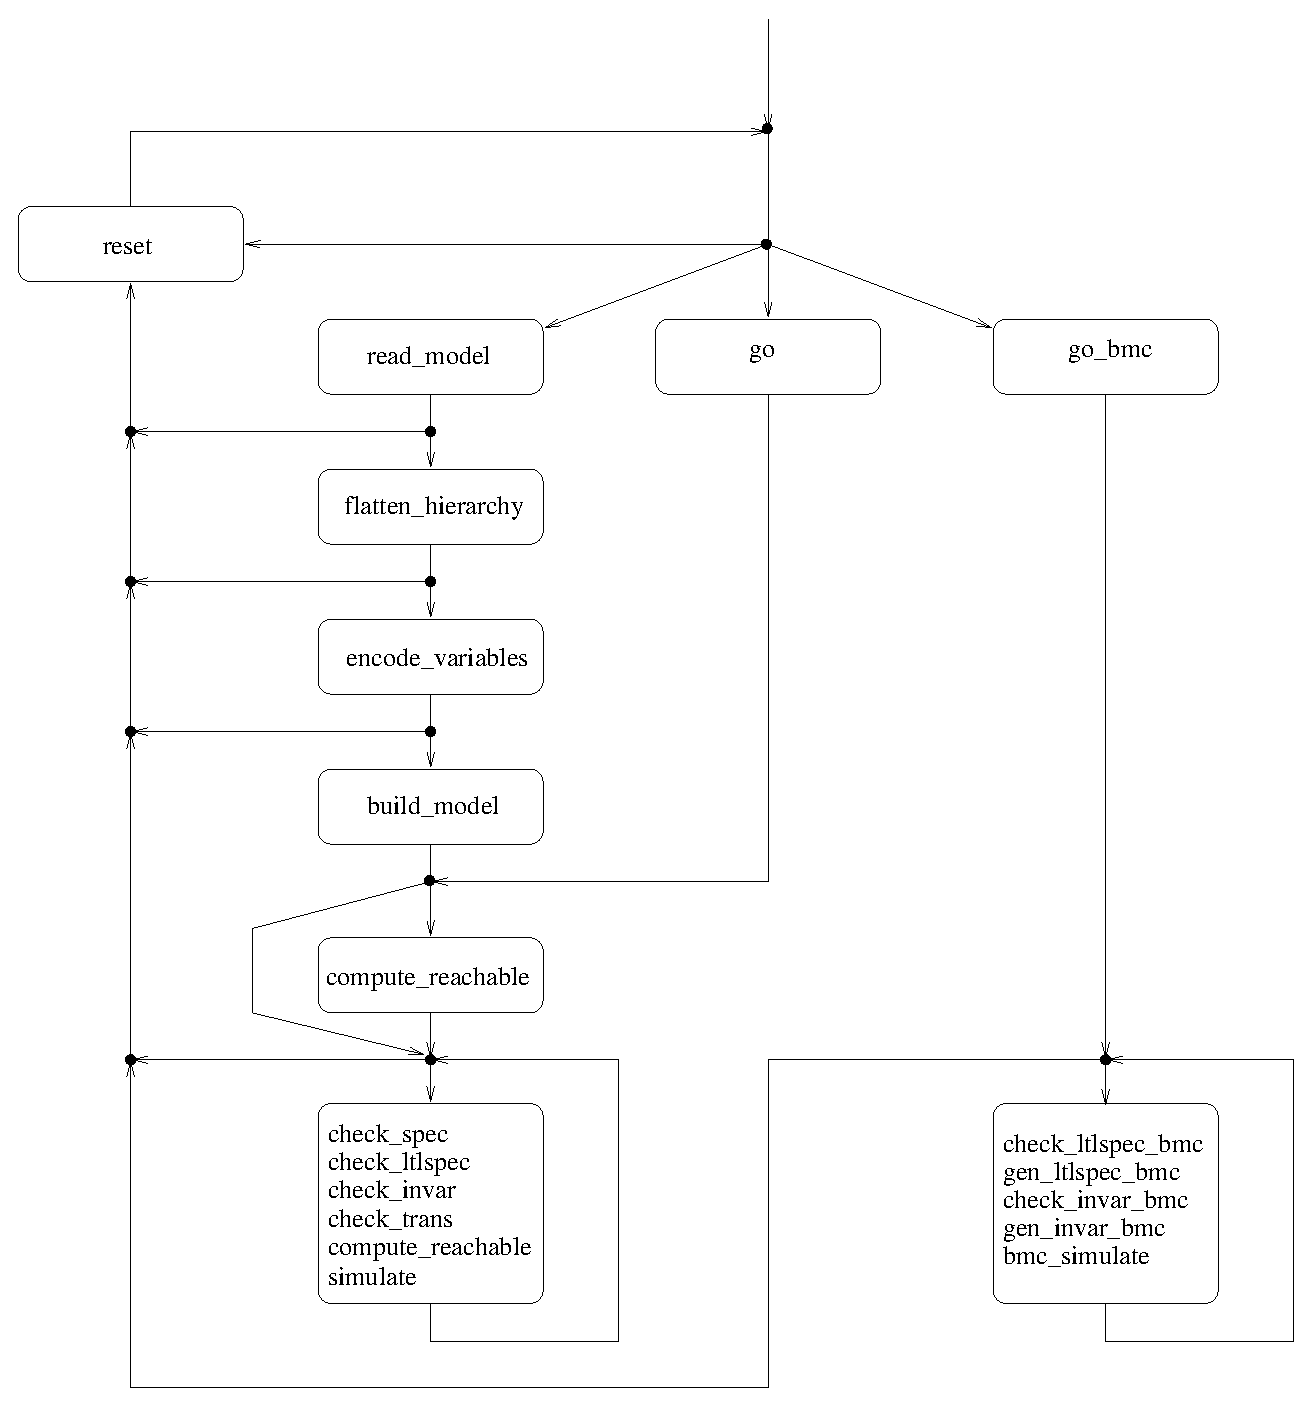
\includegraphics[width=0.8\textwidth]{cmdpo}
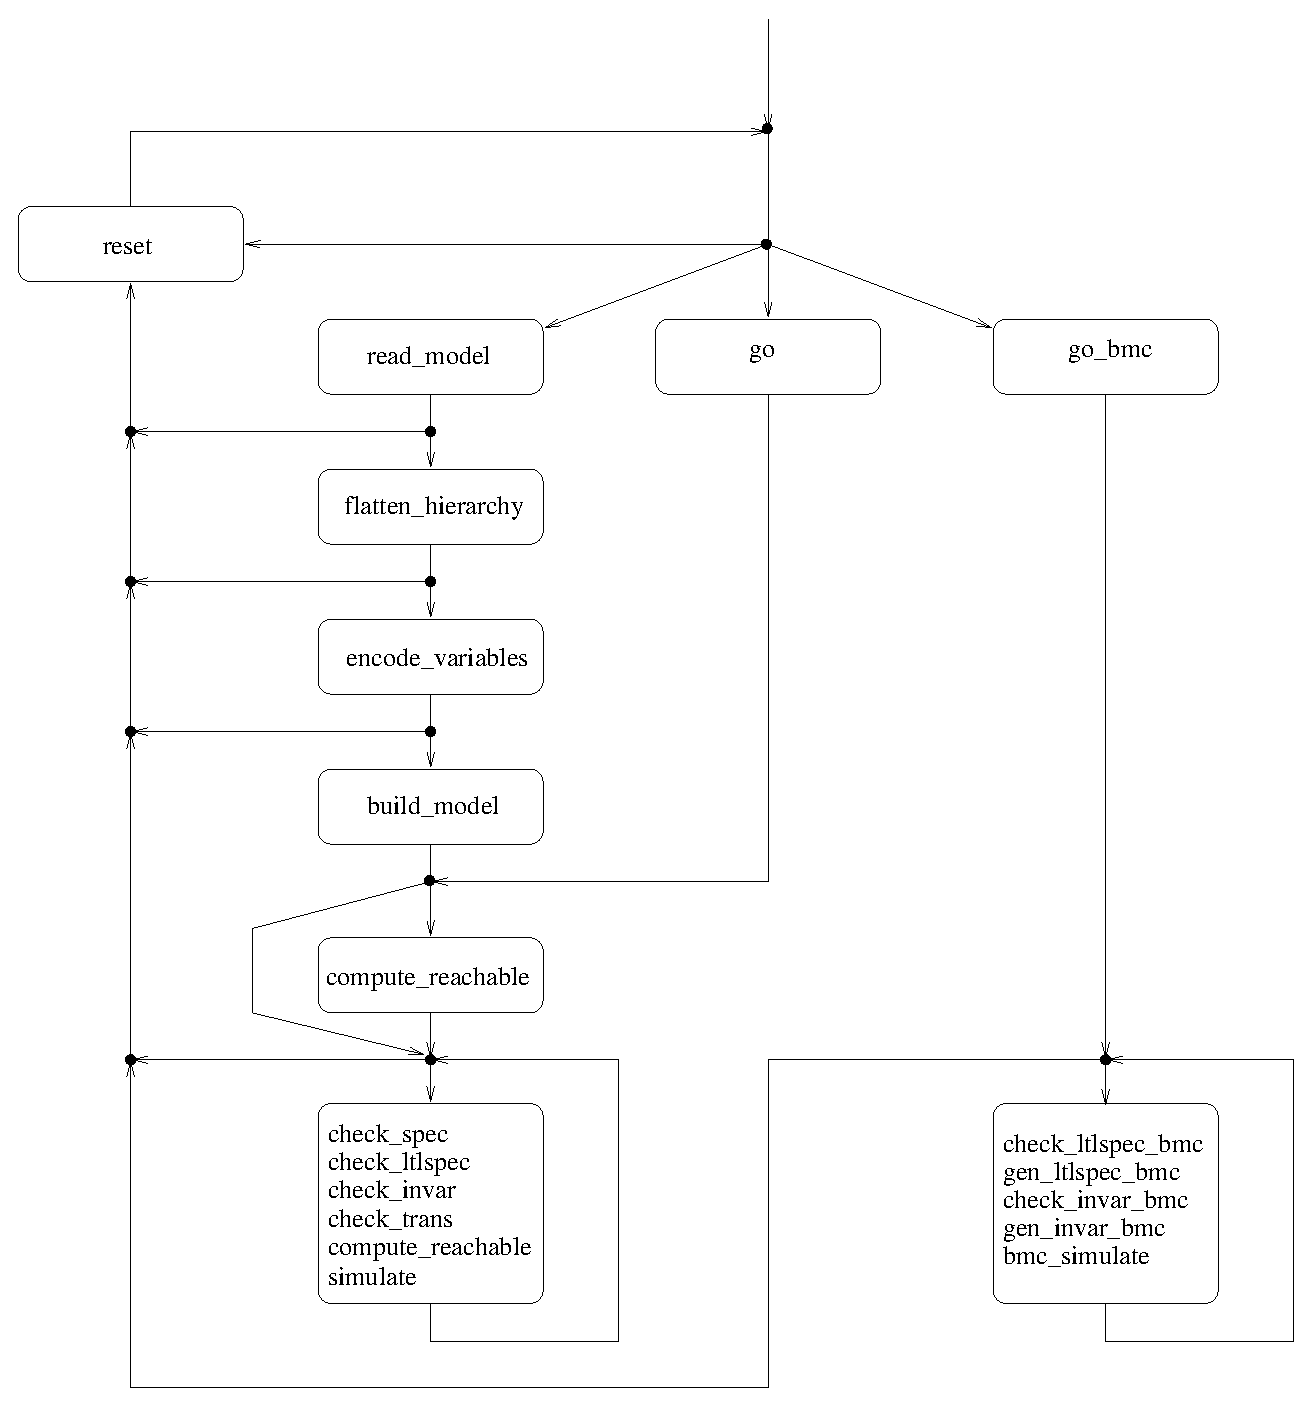
\includegraphics[width=\textwidth]{cmdpo}
\caption{The dependency among \nusmv commands.}
\end{center}
\end{figure}


\chapter{Running \nusmvhead batch}
\label{Running NuSMV batch} 
\index{options}
\index{batch, running \nusmv}
When the \commandopt{int} option is not specified, \nusmv
runs as a batch program, in the style of \smv, performing (some
of) the steps described in previous section in a fixed sequence.
\begin{alltt}
\shellprompt \shelltext{\nusmvtxt [command line options] {\it input-file}} \ret
\end{alltt}
The program described in {\it input-file} is processed, and the
corresponding finite state machine is built.  Then, if \emph{input-file}
contains formulas to verify, their truth in the specified structure is
evaluated. For each formula which is not true a counterexample is
printed.\\
The batch mode can be controlled with
the following command line options:\\
\begin{alltt}
\nusmv [-h | -help] [-v {\it vl}] [-int] [-load {\it script\_file}] [-s]
       [-cpp] [-pre {\it pps}] [-ofm {\it fm\_file}] [-obm {\it bm\_file}]
       [-lp] [-n {\it idx}] [-is] [-ic] [-ils] [-ii] 
       [-ctt] [-f] [-r] [-AG]  [-coi]
       [-i {\it iv\_file}] [-o {\it ov\_file}] [-reorder] [-dynamic] [-m {\it method}]
       [[-mono]|[-thresh {\it cp\_t}]|[-cp {\it cp\_t}]|[-iwls95 {\it cp\_t}]]
       [-noaffinity] [-iwls95preorder]
       [-bmc] [-bmc\_length {\it k}]
       [{\it input-file}]
\end{alltt}
where the meaning of the options is described below. If
{\it input-file} is not provided in batch mode, then the model is read
from standard input.\\

\begin{nusmvTable}

\opt{-help}{ }

\opt{-h}{
\index{ \code{-help}}
\index{ \code{-h}}
Prints the command line help.}

\opt{-v {\it verbose-level}}{
\index{\code{-v} {\it verbose-level}}
Enables printing of additional information on the internal operations of
\nusmv. Setting {\it verbose-level} to \code{1} gives the basic
information. Using this option makes you feel better, since otherwise
the program prints nothing until it finishes, and there is no evidence
that it is doing anything at all. Setting the {\it verbose-level}
higher than 1 enables printing of much extra information.}

\opt{-int}{
\index{ \code{-int}}
Starts interactive shell.}

\opt{-load {\it cmd-file}}{
\index{ \code{-load} {\it cmd-file}}
Interprets \nusmv commands from file {\it cmd-file}.}

\opt{-s} {
Avoids to load the \nusmv commands contained in \code{
\~/.nusmvrc} or in \code{.nusmvrc}  or in 
\code{\$\$\{\stdsyslib\}/master.nusmvrc}.} 
\vindex{\stdsyslib}
\index{master.nusmvrc}
\index{.nusmvrc}
\index{\~/.nusmvrc}

\opt{-cpp}{
\index{\code{-cpp}}
Runs preprocessor on \smv files before any of those specified with the
-pre option.}

\opt{-pre {\it pps}}{
\index{\code{-pre} {\it pps}}
Specifies a list of pre-processors to run (in the order given) on the
input file before it is parsed by \nusmv. Note that if the
\commandopt{cpp} command is used, then the pre-processors specified by
this command will be run after the input file has been pre-processed
by that pre-processor. {\it pps} is either one single pre-processor
name (with or without double quotes) or it is a space-seperated list
of pre-processor names contained within double quotes.}

\opt{-ofm {\it fm\_file}}{
\index{ \code{-ofm} {\it fm\_file}}
prints flattened model to file {\it fn\_file}}

\opt{-obm {\it bm\_file}} {
\index{ \code{-obm} {\it bm\_file}}
Prints boolean model to file {\it bn\_file}}

\opt{-lp}{
\index{\code{-lp}}
Lists all properties in \smv model}

\opt{-n {\it idx}}{
\index{\code{-n} {\it idx}}
Specifies which property of \smv model should be checked}

\opt{-is}{
\index{\code{-is}}
Does not check \code{SPEC}}

\opt{-ic}{
\index{\code{-ic}}
Does not check \code{COMPUTE}}

\opt{-ils}{
\index{\code{-ils}}
Does not check \code{LTLSPEC}}

\opt{-ii}{
\index{ \code{-ii}}
Does not check \code{INVARSPEC}}

\opt{-ctt}{
\index{\code{-ctt}}
Checks whether the transition relation is total.}

\opt{-f}{
\index{ \code{-f}}
Computes the set of reachable states before evaluating CTL expressions.}

\opt{-r}{
\index{ \code{-r}}
Prints the number of reachable states before exiting. If the \commandopt{f}
option is not used, the set of reachable states is computed.}

\opt{-AG}{
\index{ \code{-AG}}
Verifies only AG formulas using an ad hoc algorithm (see documentation for
the \envvar{ag\_only\_search} environment variable).}

\opt{-coi} {
\index{ \code{-coi}}
Enables cone of influence reduction }

\opt{-i {\it iv\_file}} {
\index{ \code{-i} {\it iv\_file}}
Reads the variable ordering from file {\it iv\_file}. }

\opt{-o {\it ov\_file}}{
\index{ \code{-o} {\it ov\_file}}
Reads the variable ordering from file {\it ov\_file}.}

\opt{-reorder}{
\index{ \code{-reorder}}
Enables variable reordering after having checked all the specification if
any.}

\opt{-dynamic}{
\index{ \code{-dynamic}}
Enables dynamic reordering of variables}

\end{nusmvTable}


\begin{nusmvTable}

\opt{-m  {\it method}} {
\index{ \code{-m} {\it method}}
Uses {\it method} when variable ordering is enabled. Possible values for
method are those allowed for the \envvar{reorder\_method} environment
variable (see \sref{Interface to DD package}).}

\opt{-mono}{
\index{ \code{-mono}}
Enables monolithic transition relation}

\opt{-thresh {\it cp\_t}}{ 
\index{ \code{-thresh} {\it cp\_t}}
conjunctive partitioning with threshold of each
partition set to {\it cp\_t} (DEFAULT, with {\it cp\_t}=1000)}

\opt{-cp {\it cp\_t}}{
\index{ \code{-cp} {\it cp\_t}}
DEPRECATED: use \command{thresh} instead.}

\opt{-iwls95 {\it cp\_t}}{
\index{ \code{-iwls95} {\it cp\_t}}
Enables Iwls95 conjunctive partitioning and sets
the threshold of each partition to {\it cp\_t}}

\opt{-noaffinity}{
\index{ \code{-noaffinity}}
Disables affinity clustering }

\opt{-iwls95preoder} {
\index{ \code{-iwls95preorder}}
Enables \Iwls preordering}

\opt{-bmc} {
\index{ \code{-bmc}}
Enables BMC instead of BDD model checking }

\opt{-bmc {\it k}}{
\index{ \code{-bmc} {\it k}}
Sets \envvar{bmc\_length} variable, used by BMC}

\end{nusmvTable}





% Just to include all citations 
\nocite{BCCZ99}
\nocite{CCG+02}
\nocite{CCGR00}
\nocite{BCLM+94}
\nocite{CGH97}
\nocite{CMB90}
\nocite{Dil88}
\nocite{McMil92}
\nocite{McMil93}
\nocite{Mart85}
\nocite{MOON00}
\nocite{EMSS91}
\nocite{RAP+95}
\nocite{Som98}
\nocite{Vis96}


% Print bibliography here.
\bibliography{main}

\newpage
\appendix
\chapter{Compatibility with CMU \smv}
The \nusmv language is mostly source compatible with the original
version of \smv distributed at Carnegie Mellon University from
which we started.  In this appendix we describe the most common
problems that can be encountered when trying to use old CMU
\smv programs with \nusmv.

The main problem is variable names in old programs that conflicts with
new reserved words.  The list of the new reserved words of \nusmv
w.r.t. CMU \smv is the following:

\begin{table}[h]
\begin{tabular}{p{100pt}p{300pt}}
\code{F, G, X, U, V, W, H, O, Y, Z, S, T, B} &
These names are reserved for the LTL temporal operators.\\
\code{LTLSPEC} &
It is used to introduce LTL specifications. \\
\code{INVARSPEC} &
It is used to introduce invariant specifications.\\
\code{IVAR} &
It is used to introduce input variables. \\
\code{JUSTICE} &
It is used to introduce ``justice'' fairness constraints.\\
\code{COMPASSION} &
It is used to introduce ``compassion'' fairness constraints. \\
\end{tabular}
\end{table}

The \code{IMPLEMENTS}, \code{INPUT}, \code{OUTPUT} statements are not
supported by \nusmv. They are parsed from the input file, but 
are internally ignored.

\nusmv differs from CMU \smv also in the controls that are
performed on the input formulas. Several formulas that are valid for CMU
\smv, but that have no clear semantics, are not accepted by 
\nusmv. In particular:

\begin{itemize}
\item It is no longer possible to write formulas containing nested
`\code{next}'.
\begin{alltt}
TRANS
  next(alpha & next(beta | next(gamma))) -> delta
\end{alltt}
\item It is no longer possible to write formulas containing
`\code{next}' in the right hand side of ``normal'' and ``init''
assignments (they are allowed in the right hand side of ``next''
assignments), and with the statements `\code{INVAR}' and
`\code{INIT}'.
\begin{nusmvCode}
INVAR
  next(alpha) & beta
INIT
  next(beta) -> alpha
ASSIGN
  delta := alpha & next(gamma);       -- normal assignments
  init(gamma) := alpha & next(delta); -- init assignments
\end{nusmvCode}
\item It is no longer possible to write `\code{SPEC}',
`\code{FAIRNESS}' statements containing `\code{next}'.
\begin{nusmvCode}
FAIRNESS
 next(running)
SPEC
 next(x) & y
\end{nusmvCode}
\item The check for circular dependencies among variables has been 
done more restrictive.
We say that variable {\it x} depends on variable {\it y} if {\it x := f(y)}.
We say that there is a circular dependency in the definition of {\it x} if:
\begin{itemize}
\item  {\it x} depends on itself ( e.g. {\it x := f(x,y)} );
\item {\it x} depends on {\it y} and {\it y} depends on {\it x} (e.g. {\it x :=
f(y)} and {\it y := f(x)} or {\it x := f(z)}, {\it z := f(y)} and {\it y :=
f(x)} ).
\end{itemize}
In the case of circular dependencies among variables there is no fixed
order in which we can compute the involved variables. Avoiding circular
dependencies among variables guarantee that there exists an order in
which the variables can be computed. In \nusmv circular
dependencies are not allowed.

In CMU \smv the test for circular dependencies is able to detect
circular dependencies only in ``normal'' assignments, and not in ``next''
assignments. The circular dependencies check of \nusmv has been
extended to detect circularities also in ``next'' assignments. For
instance the following fragment of code is accepted by CMU \smv
but discarded by \nusmv.
\begin{nusmvCode}
MODULE main
VAR
  y : boolean;
  x : boolean;
ASSIGN
  next(x) := x & next(y);
  next(y) := y & next(x);
\end{nusmvCode}
\end{itemize}

Another difference between \nusmv and CMU \smv is in the variable
order file.  The variable ordering file accepted by \nusmv can be
partial and can contain variables not declared in the model. Variables
listed in the ordering file but not declared in the model are simply
discarded. The variables declared in the model but not listed in the
variable file provided in input are created at the end of the given
ordering following the default ordering. All the ordering files
generated by CMU \smv are accepted in input from \nusmv but the
ordering files generated by \nusmv may be not accepted by CMU \smv.
Notice that there is no guarantee that a good ordering for CMU \smv is
also a good ordering for \nusmv.  In the ordering files for \nusmv,
identifier \code{\_process\_selector\_} can be used to control the
position of the variable that encodes process selection. In CMU \smv
it is not possible to control the position of this variable in the
ordering; it is hard-coded at the top of the ordering.


\cleardoublepage

% Print Indices here 
\printindex[com]
\printindex[var]
\printindex

\end{document}
\endinput
